\newcommand{\NbasesV}{\textit{N}}
\newcommand{\Nbases}{6}
\newcommand{\Nml}{6}
\newcommand{\NmlT}{5}
\newcommand{\NmlA}{2}
\newcommand{\Ncb}{4}
\newcommand{\MML}{método multirrótulo}
\newcommand{\MMLs}{métodos multirrótulo}
\newcommand{\MRLM}{Recursive Dependent Binary Relevance}
\newcommand{\MRLMa}{RDBR}

\newcommand{\legendaTab}[2]{Desempenho dos métodos multirrótulos com \textit{#2} medido pela métrica \textit{#1} }
\newcommand{\jqo}{J48}
\newcommand{\EBA}{Example Based Accuracy}
\newcommand{\SA}{\textit{Subset Accuracy}}
\newcommand{\HL}{\textit{Hamming Loss}}
\newcommand{\CC}{\textit{Classifier Chain}}
\newcommand{\ECC}{\textit{Ensemble of }~\CC}

\chapter{Introdução}
Segundo \cite{rezende2003sistemas} Aprendizado de Máquina é uma área de Inteligência Artificial
cujo objetivo é o desenvolvimento de técnicas computacionais
sobre o aprendizado bem como a construção de sistemas capazes de adquirir
conhecimento de forma automática. Essa área tem atraido a atenção de muitos 
pesquisadores em diversas especialidades. Dentro dessa área, encontra-se a subárea Aprendizado Supervisionado.
Em Aprendizado Supervisionado, um problema de classificação é a tarefa de encontrar
uma técnica capaz de predizer a classe ou as classes que uma instância de
um objeto em específico pertence \cite{rezende2003sistemas}.
Para completar essa tarefa, a técnica deve usar exemplos de treino cujas as classes
são conhecidas que lhe são dispostas. Uma instância é um objeto do mundo real descrito
por um vetor de valores numéricos ou nominais e por um conjunto de rótulos.
Na literatura, as classes também são chamadas de rótulos (REZENDE, 2003, p. 91)
e quando as instâncias só podem assumir um único rótulo, o problema é chamado de classificação unirrótulo,
do contrário, é chamado de problema de classificação multirrótulo (BORGES, 2012).

Problemas de classificação multirrótulo estão presentes em diversas áreas, trabalhos relevantes podem
ser encontrados em áreas como a bioinfomática, diagnóstico médico, classificação de imagens e principalmente
categorização de textos (CARVALHO, 2009, p. 2). A classificação multirrótulo é inevitavelmente
mais complexa que a unirrótulo. Para solucioná-la,  o método multirrótulo mais conhecido é um método simples chamado de
Relevância Binária (BR – Binary Relevance) (READ, 2011, p. 2). 
Há muitas críticas sobre o método, sendo a maior delas a incapacidade do método de reconhecer correlação entre os rótulos (READ, 2011, p. 2).
Com o intuito de alcançar melhores resultados que o BR, alguns autores o aprimoraram ou elaboraram novos tipos de métodos
de tal forma que divergem na forma como resolvem o problema (READ, 2011). 
Por exemplo, existem métodos que transformam o problema multirrótulo em
diversos problemas unirrótulo, como é o caso do BR, e outros métodos que são classificadores especiais, capazes de classificar diretamente sobre os problemas multirrótulo, sem necessidade de transformação, como é o caso do Multi-Label C4.5 (MADJAROV et al., 2012, p. 5). 

Com tantos métodos novos, alguns deles apresentados por Carvalho (2009)
e por Read(2011) é necessário realizar comparações e testes de qualidade.
É certo que já existem análises e comparações entre os métodos,
no entanto há necessidade de avaliar os métodos de forma mais formal
e reforçar as conclusões alcançadas pelos autores dos métodos além de elaborar
uma forma eficiente de comparar tipos diferentes de métodos multirrótulos (DRUMMOND, 2008).

\section{Motivações}
% A análise dos métodos multirrótulo traz os seguintes benefícios:
O melhor entendimento do funcionamento dos métodos multirrótulo permite:
\begin{itemize}
 \item descobrir atributos destes que se alterados, aproveitados
 e/ou combinados podem acarretar na criação de novos métodos e/ou na melhora dos existentes.
 \item prever, com uma certa taxa de erro, seus desempenhos, o que facilita o uso mais inteligente dos métodos
 sem precisar utilizar muito esforço computacional devido a testes.
 \item reforçar ou contrariar as conclusões já estabelecidas dos métodos, uma vez que a maioria delas são 
 baseadas em testes experimentais.
\end{itemize}

\section{Objetivos}
O objetivo geral deste trabalho é analisar e comparar métodos multirrótulos distintos e 
desenvolver um novo algoritmo de classificação multirrótulo.
Mais formalmente, a análise deve implicar em conclusões matemáticas ou estatísticas sobre o desempenho dos métodos multirrótulo.
O Objetivo geral pode ser detalhado nos seguintes objetivos específicos:
\begin{itemize}
 \item Descobrir como medir correlação entre rótulos;
 \item Comparação estatística e análise crítica dos métodos multirrótulos;
 \item Elaboração de um algoritmo de um novo método multirrótulo;
 \item Implementação dos métodos multirrótulos em uma biblioteca que integra técnicas de reconhecimento de padrões.
\end{itemize}


% \section{Contribuições}
\section{Estrutura do Trabalho}
O restante do trabalho está organizado da seguinte forma:
\begin{itemize}
 \item O capítulo 2 apresenta os principais conceitos da classificação multirrótulo, bem como
 os métodos usados para avaliação de desempenho de classificadores multirrótulo.
 \item O capítulo 3 apresenta a definição de diferentes métodos de classificação multirrótulo usados neste trabalho,
 bem como suas complexidades algorítma.
 \item O capítulo 4 apresenta a definição de um novo método de classificação multirrótulo proposto neste trabalho.
 \item O capítulo 5 começa apresentando as configurações experimentais escolhidos para realização de testes e termina
 apresentando os resultados e a sua análise detalhada.
 \item No capítulo 6 são apresentados as conclusões finais sobre o desempenho dos métodos e sobre a análise do capítulo anterior.
\end{itemize}


\chapter{Classificação multirrótulo}

Problemas de classificação estão situadas na área de aprendizado supervisionado, que por sua vez é uma 
subárea da mineração de dados. Para \cite{dunham2003introductory} a mineração de dados é definido como a descoberta
de informações escondidas em um conjunto de dados. Ela surgiu diante do grande crescimento de dados armazenados
em arquivos de computadores e do desejo dos usuários desses dados em obter informações mais detalhadas do que simplesmente
os próprios dado em si. A mineração de dados tem por objetivo satisfazer o desejo desses usuários ao desenvolver técnicas
capazes de explicitar informações valiosas, antes escondidas ao usuários diante de uma alta quantidade de dados.
Uma de suas subáreas é a aprendizado supervisionado. Nela, segundo \cite{mohri2012foundations},
os dados pelos quais deve-se extrair as informações são associados a uma variável especial cujo valor
é conhecido e a técnica deve predizer os rótulos
corretamente para novos dados cujo valor da variável especial associada a elas é desconhecido.

Normalmente, em aprendizado supervisionado os dados são objetos de um domínio específico e cada um dos objetos
é descrito por um conjunto fixo de atributos \cite{rezende2003sistemas}. 
Esses objetos são usualmente chamados de instâncias ou exemplos do domínio do problema.
Um atributo é uma descrição de uma característica da instância.
Por exemplo, de um do ponto de vista médico??.
Em problemas de classificação unirrótulo, a variável especial associada a cada instância é discreta
e é chamada de classe ou rótulo. A técnica que prediz as classes é chamado de classificador.
% cada exemplo do objeto do domínio em questão é associado 
% a um único rótulo e o objetivo é desenvolver um sistema classificativo que consiga predizer corretamente
% o rótulo. 
Na classificação multirrótulo, cada instância pode assumir um ou mais rótulos, e a técnica
que prediz os rótulos de uma instância é chamada de classificador multirrótulo.
Por exemplo, uma instância de filme pode ser rotulado como sendo de romance e comédia, 
e não exclusivamente de romance ou comédia.

Assim a classificação é a tarefa de encontrar um classificador capaz de predizer 
o rótulo ou os rótulos de uma instância corretamente.
Para completar essa tarefa, o classificador deve usar dados de entrada que são exemplos
de treino cujos rótulos são conhecidos afim de
reconhecer e aprender padrões.

\section{Enunciado do problema}

Em um problema de classificação multirrótulo, seja $X$ o espaço de características tal que
$X\subseteq \mathbb{R}^n$ e $L=\{l_1,l_2,l_3,...l_r\}$ o conjunto dos $r$ rótulos possíveis do problema,
uma instância é definida como sendo uma dupla de vetores $(x',y')$ tal que $x'\in X$ e $y'$ é um vetor binário
$y'=(y'_1,y'_2,...,y'_r)$ de tal forma que $y'_i=1$ indica a presença do rótulo $l_i$ na instância.
Assim, o espaço de rótulos possíveis para uma instância qualquer é definido como $Y=\{0,1\}^r$.
% A transformação de um vetor binário pertencente ao espaço $Y$ para o conjunto de rótulos correspondente,



A tarefa do problema de classificação multirrótulo é encontrar uma função $C : X \rightarrow Y$ de forma
a maximizar uma métrica de qualidade, definida por uma função que mapeia as predições da função $C$
e os rótulos reais alvos a um valor numérico entre $0$ a $1$.
A função $C$ é estimada a partir de uma base de treino $D=\{(x_1,y_1),(x_2,y_2),...,(x_n,y_n)\}, x_i\in X, y_i\in Y$.

Note que em um problema de classificação unirrótulo todas as instâncias da forma $(x',y')$ tem como $y'$
um vetor binário de rótulos onde apenas uma posição tem valor $1$. Assim, podemos ver o problema classificação
unirrótulo como um caso específico do problema de classificação multirrótulo.
Outro ponto importante a notar é a grande diferença da complexidade da classificação unirrótulo para a multirrótulo.
Enquanto que na classificação unirrótulo o número de possíveis rotulações que uma instância desconhecida pode ter é
$r$, linear em relação ao número de rótulos, na multirrótulo o número cresce exponencialmente, a saber, $2^r$.
Assim construir um classificador multirrótulo é mais complexo que um classificador unirrótulo.



\section{Avaliação de Desempenho}
\begin{verbatim}
ESBOÇO:
-Apresentar matematicamente o que pode indicar correlação entre rótulos e outras coisas
conforme o artigo: "Bayes Optimal Multilabel Classification via Probabilistic Classifier Chains".
-Falar que é diferente do multiclasse e a razao disso
\end{verbatim}

A avaliação de desempenho de classificadores, tanto multirrótulo quanto unirrótulo, é comumente feito
por meio de testes nas amostras coletadas do problema.
Isso é feito corretamente com a ajuda de métodos de reamostragem fundamentados pela ciência estatística,
descritas na seção \ref{sec:modelav}.

A avaliação de desempenho dos classificadores multirrótulos se difere da unirrótulo principalmente na
quantificação da qualidade de predição. Enquanto que na classificação unirrótulo existe somente uma classificação
correta dentre apenas $r$ possíveis classificações, na classificação multirrótulo podem existir mais de uma combinação, 
dentre as $2^r$ possíveis, que estejam corretas ou parcialmente corretas.
Para isso, são definidas várias métricas multirrótulo na seção \ref{sec:metrics},
cada uma capturando um aspecto diferente do desempenho do classificador. 



\subsection{Métricas}
Seja $P=(p_1,p_2,...,p_n), p_i \subseteq L$
% $\hat{y}=(\hat{y}_1,\hat{y}_2,...,\hat{y}_n), \hat{y}_i \in Y$
um vetor de predições de rótulos produzido pela
classificação das $n$ instâncias de rótulos $(r_1,r_2,...,r_n), r_i \subseteq L$
% da base $D=\{(x_1,y_1),(x_2,y_2),...,(x_n,y_n)\}, x_i\in X, y_i\in Y$
respectivamente. Note que aqui as predições $p_i$ e os rótulos $r_i$ estão representados na forma de conjunto de rótulos,
e não na forma de vetor binário.
As métricas multirrótulo propostas servem para quantificar a qualidade de $P$
e úteis para resumi-lo a um único valor escalar entre 0 e 1.
Abaixo estão algumas métricas definidas por \cite{reviewml2013}:
\label{sec:metrics}
\subsubsection{Hamming Loss}
\begin{equation}
 hloss(P)=\frac{1}{n} \sum_{i=1}^n{|p_i \triangle r_i|}
\end{equation}
O símbolo $\triangle$ é definido como a diferença simétrica entre dois conjuntos de mesmo tamanho.
O \textit{Hamming Loss} significa a proporção de rótulos preditos mal classificados. Por rótulo predito mal classificado
entende-se que classificou um rótulo que não existia ou deixou de classificar um rótulo relevante.
Note que quanto menor o seu valor, melhor é a qualidade de predição, sendo que 0 é a qualidade perfeita e 1 a mais
imperfeita possível.

Em \cite{pcc2010} é mostrado que para que um classificador minimize o valor dessa métrica, basta minimizar
o erro (mal classificação) para cada rótulo individualmente. 
Assim, para minimizar essa métrica não é necessário levar
em consideração a correlação entre rótulos. Dessa forma considerar os rótulos de forma independente é o suficiente para minimizá-lo,
apesar de que um método multirrótulo pode usar a correlação entre rótulos para ajudar a minimizá-lo, uma vez que 
a tarefa de classificação, mesma que de forma independente, é difícil.

\subsubsection{Subset Accuracy}
\subsubsection{Example Based Accuracy}
\subsubsection{Precision}
\subsubsection{Recall}
\subsection{Modelo de Avaliação}
\label{sec:modelav}

\chapter{Métodos Multirrótulos}
\section{Transformação do Problema}
\subsection{Relevância Binária - BR}
\label{sec:br}


O método da Relevância Binária, conhecido como \textit{Binary Relevance} \cite{br2010}, 
é composto de $r$ classificadores binários $c_1,c_2,...,c_r$. Cada classificador $c_i$ 
é associado ao rótulo $i$ e treinado com o único objetivo de resolver
um problema de classificação binária onde as instâncias que
tem o rótulo $r_i$ são consideradas para o classificador $c_i$ como positivas
e as demais instâncias como
negativas. 
Após todos os classificadores terem sido treinados, quando uma instância
ainda não de rótulo desconhecido 
é apresentado aos classificadores, todos aqueles que produzirem uma classe positiva
terão sua classe associada á nova instância.
O método de classificação de relevância binária é uma estratégia de transformação do
problema, que decompõe o problema de classificação multirrótulo em diversos problemas
de classificação binária unirrótulo, um para cada um dos rótulos do problema.

\begin{figure}
 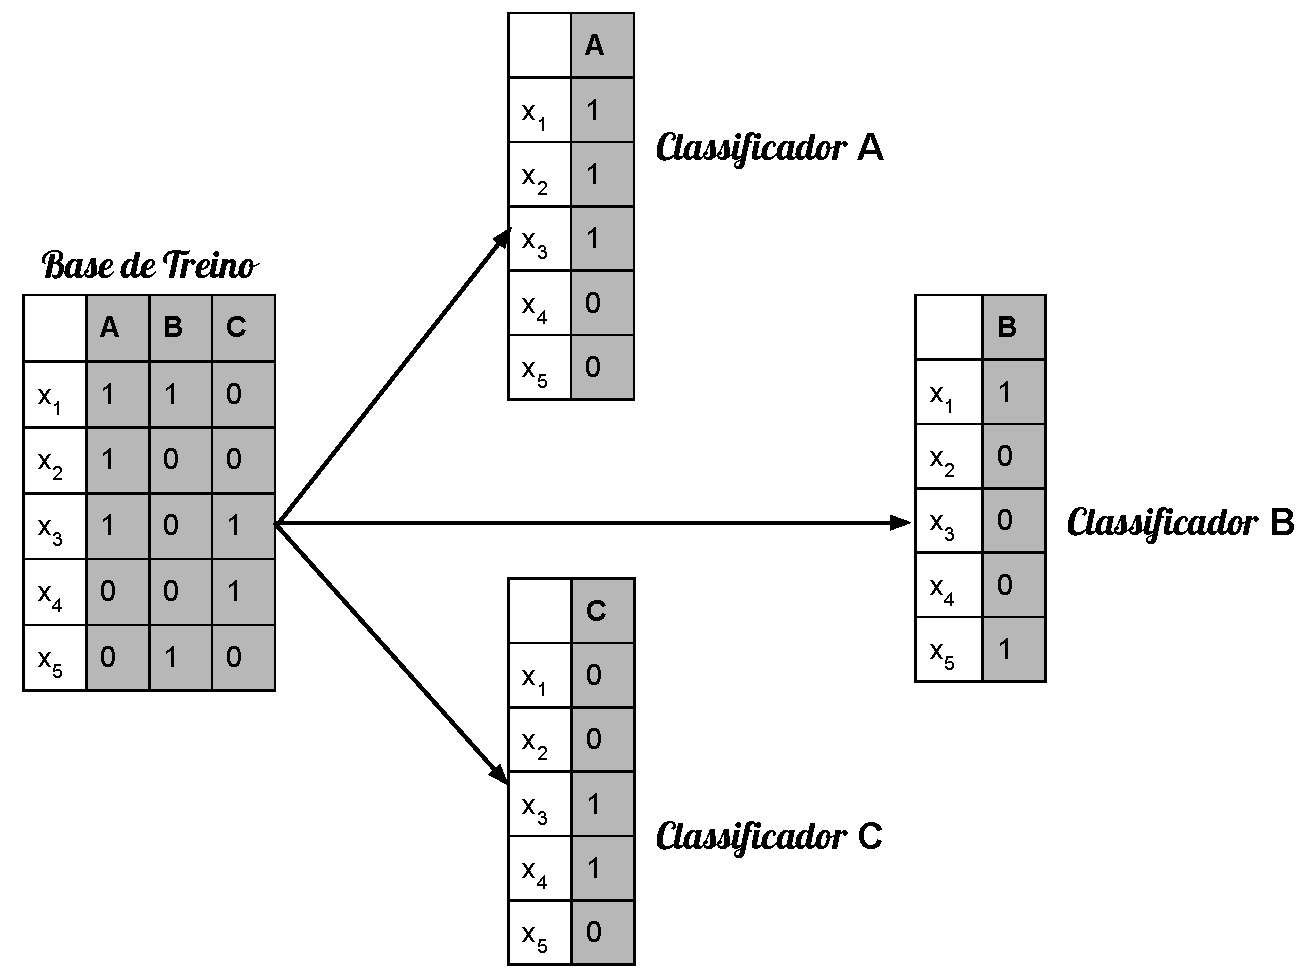
\includegraphics[width=1\linewidth]{BR-figure2}
 
 \caption{Exemplo da transformação realizada pelo método \textit{BR}}
\label{fig:br}

\end{figure}

A figura \ref{fig:br} ilustra um exemplo da transformação que o BR realiza em um problema multirrótulo
de rótulos $A,B$ e $C$ e 6 instâncias. Nele vemos que o BR transforma a base de treino em 3 novas bases
de dados, um para cada classificador binário.





\subsection{Classifier Chain}


A idéia básica desse algoritmo é semelhante ao BR: realiza a transformação do
problema multirrótulo decompondo-o em diversos problemas
de classificação binária unirrótulo, um para cada um dos rótulos do problema.
Ele é também composto de $r$ classificadores binários $c_1,c_2,...,c_r$ e cada um
é associado a um único rótulo distinto. A diferença do \textit{Classifier Chain} para o BR está
em que os classificadores binários estão organizados em uma cadeia de tal forma que
o classificador $c_i$ é contruído com base nos rótulos ou predições dos classificadores anteriores
($c_{i-1},c_{i-2},...,c_{1}$) \cite{cc2009}. O classificador $c_i$ não está necessariamente associado ao rótulo $r_i$,
ele pode estar associado a qualquer um dos rótulos.
Essa associação é feita de forma aleatória ou pré-definida por parâmetro do algoritmo.

Na fase de treinamento do método o espaço de características de cada classificador $c_i$ é 
extendido com os valores dos $i-1$ rótulos reais anteriores da cadeia. Veja um exemplo 
ilustrado na figura \ref{fig:CCtraintest} onde o método é treinado sobre uma base de treino de três rótulos ($A,B,C$)
e seis instâncias. Note que a base de treino do classificador binário $B$ tem como característica adicional o rótulo $A$.

Na fase de predição do método a classificação ocorre de forma sequencial, na ordem em que a cadeia foi definida.
O classificador $c_1$ inicia o processo de classificação realizando a estimativa do rótulo associado da instância teste.
A partir daí o classificador $c_i$ realiza a predição da instância teste assim que a predição do classificador $c_{i-1}$
esteja disponível. O classificador $c_i$ agrega a predição do classificador $c_{i-1}$, que é um valor binário (0 ou 1),
a instância de teste. A figura \ref{fig:CCtraintest} ilutra bem o processo de predição na qual o vetor de características da
instância teste vai crescendo com adição de cada estimativa de rótulo.


\begin{figure}

 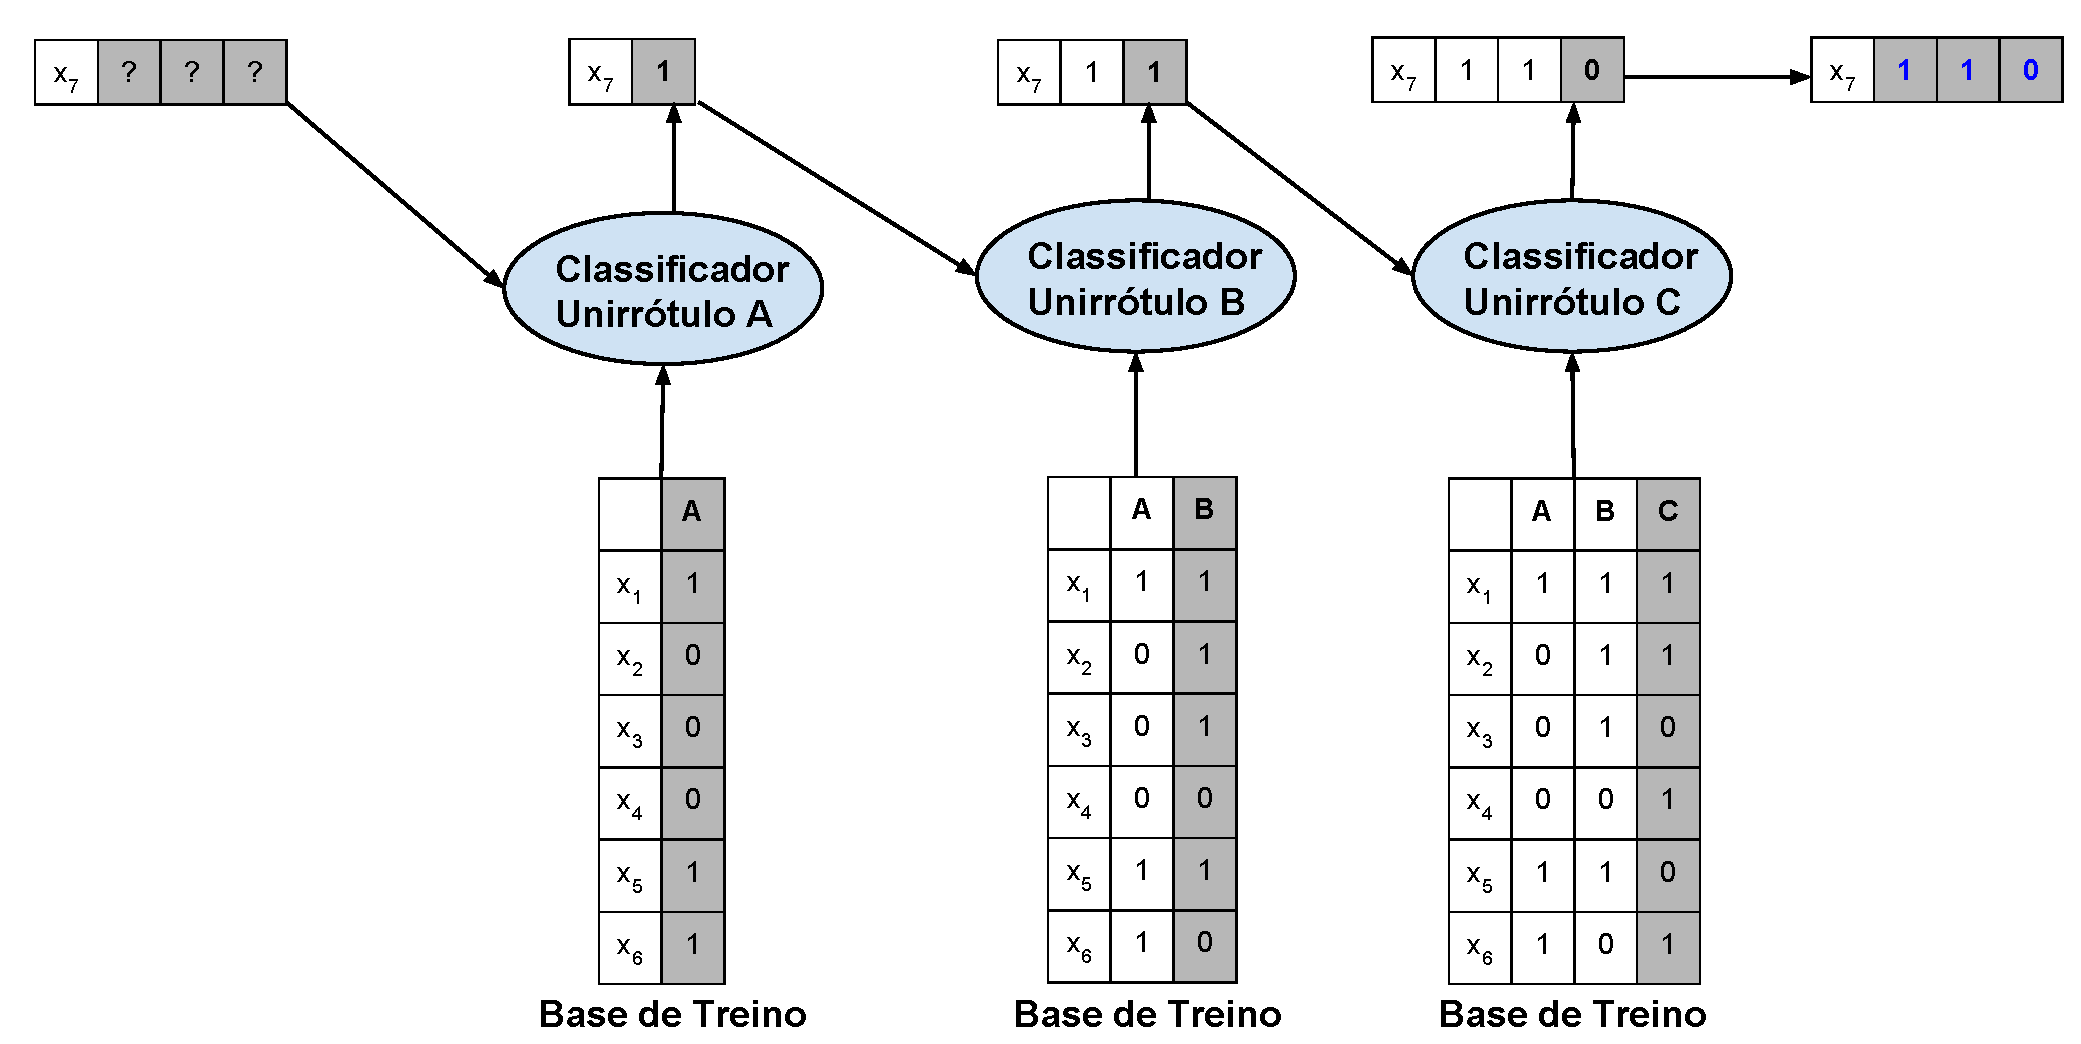
\includegraphics[width=1\linewidth]{CC-train-test}
 \caption{Ilustração de um exemplo da fase de treinamento e de predição do método Classifier Chain.}
\label{fig:CCtraintest}
\end{figure}


\subsection{Ensemble of Classifier Chain}
\subsection{Probabilistic Classifier Chain}
\subsection{Relevância Binária Dependente - DBR}
\label{sec:dbr}
Este método é proposto por \cite{dbr2014} é baseado no método BR
e a diferença entre ambos está no fato de 
que o DBR considera dependência entre os $r$ rótulos.

O DBR é composto de dois classificadores multirrótulo, $c_0$ e $c_1$ , 
cada um composto de $r$ classificadores binários. O classificador multirrótulo $c_0$ é
exatamente o método BR. Os $r$ classificadores binários $c_1^1,c_1^2...,c_1^r$ que compoêm $c_1$ 
  trabalham em um novo espaço de características $X^{new}=X \times \{0,1\}^{r-1}$.
  Esse novo espaço é a extensão do antigo com a adição de $r-1$ rótulos.
  Digamos que $(x,y)$ seja uma instância do espaço original $X \times Y$
  onde $x \in X$ e $y \in {\{0,1\}}^{r}$, então cada instância
  do classificador binário $c_1^i$ tem $|x|+r-1$ características
  e é definido como sendo $(x,y_1,...,y_{i-1},y_{i+1},...,y_{r})$.
  
  \subsubsection{Fase de Treinamento}
  Dado uma base de dados de treino $D=\{((x_i),y_i)|i=1,...,n\}$ onde $x_i \in X$ é o vetor de características de cada instância
  e $y_i \in Y$ o vetor binário de rótulos de cada instância,
  primeiro treina-se o $c_0$
  no espaço de características original conforme o treinamento do próprio BR mostrado na seção \ref{sec:br}.
  Depois, treina-se $c_1$ em uma nova base de dados $D'$ que é construída a partir de $D$ adicionando os rótulos de cada
  exemplo como características. Assim, $D'$ é composta pelos exemplos $\{((x_i,y_i),y_i) |i=1,...,n\}$ e
  cada classificador binário $c_1^j$ de $c_1$ é induzido na base de dados $D'_j=\{(x_i,y_{i,1},...,y_{i,j-1},y_{i,j+1},...,y_{i,r}),y_{i,j} | i=1,...,n\}$.
  Note que a característica representando o $j$-ésimo rótulo é removido da base de dados.
  Dessa forma, ao invés de estimar apenas $P(y_j|x)$ como o BR faz, o método é capaz de detectar dependência entre os rótulos ao
  estimar $P(y_j|x,y_1,...,y_{j-1},y_{j+1},...,y_r)$.
  
  \subsubsection{Fase de Predição}
  Como no caso do Classifier Chain, os rótulos reais $y$, que são usado como características adicionais em cada instância de treino,
 estão disponíveis apenas durante a fase de treinamento.
 Com isso, para tornar possível a classificação por $c_1$, o DBR usa o classificador $c_0$ com a finalidade de
 estimar os rótulos, %  Para alcançar isso, o \MRLMa~, após treinado, usa $c_0$ para realizar as primeiras estimativas dos rótulos,
 o que resulta no predição $c_0(x)=\hat{y}=(\hat{y}_1,\hat{y}_2,...,\hat{y}_r)$, que servirá como parte da instância de $c_1$,
 onde antes era o lugar de $y$. 
 A partir daí, $c_1$ classifica o vetor de características $(x,\hat{y})$ de uma forma bem similar ao BR:
 cada classificador binário $c_1^i$ do método é responsável pela predição de um único rótulo da instância
 cujo vetor de características é $(x,\hat{y}_1,...,\hat{y}_{j-1},\hat{y}_{j+1},...,\hat{y}_r)$.

\subsection{Monte Carlo Classifier Chain}
\cite{mcc2012}

% \section{Adaptação de classificadores}
% \subsection{ML-KNN}
% \subsection{Rede Neural Artificial}
% \subsection{C4.5 multirrótulo}
% \subsection{CRankSVM}
% \subsection{MAIS...}


\chapter{Recursive Dependent Binary Relevance - RDBR}
A proposta de \MRLM~(\MRLMa)~é fundamentada no \MML~\textit{dependent binary relevance} (DBR) \cite{dbr2014}, que é explicado
na seção \ref{sec:dbr}. Assim como o DBR e o CC, o \MRLMa~é um método baseado na transformação do problema que dividem o problema
multirrótulo em vários problemas classificação binária. Todos eles exploram a correlação entre os rótulos por meio da adição de
características especiais que representam os rótulos reais ou estimativas dos rótulos reais ao espaço de características original. 
Mas, diferentemente dos outros, o \MRLMa~adiciona uma inteligência no uso dessas características especiais na fase de predição do método.
A forma de como isso é feito, bem como o funcionamento completo do algoritmo de classificação e a fundamentação teórica
do \MRLMa~são detalhados na seção \ref{sec:mrlm_algo}. 
A seção \ref{sec:mrlm_analise} analisa o funcionamento e o desempenho do \MRLMa~de forma empírica.


\section{Algoritmo de \MRLM~-~\MRLMa}
\label{sec:mrlm_algo}
Como foi dito anteriormente, o \MRLM~é baseado no DBR. 
% Ambos se baseiam na expansão do espaço de características
% com características que representam a estimativas dos rótulos como forma de explorar
% a correlação entre rótulos. Isso é feito usando a predição do BR no espaço de características original.
% Ou seja, 
Ambos dependem da hipótese de que as estimativas dos rótulos em $Y$ por um classificador multirrótulo $c_0$
são boas características para aprimorar as estimativas dos mesmos rótulos por um novo classificador $c_1$
e que quanto melhor forem as estimativas dos rótulos por $c_0$, melhores são as de $c_1$.
% Nesse caso, podemos dizer
% que o classificador $c_0$ é usado por $c_1$ como parâmetro para .
E ainda ambos usam o BR como classificador multirrótulo base, que servirá para realizar as primeiras estimativas dos 
rótulos.

No entanto, o \MRLMa, ao invés de usar apenas o classificador base $c_0$ como função para contruir
as características adicionais que o $c_1$ usa, como o DBR,
ele também usa o próprio $c_1$ para essa finalidade, ou seja, há uma atualização das estimativas das características
pelo próprio classificador que as usam.
A idéia é que cada vez que $c_1$ as atualiza, melhores ficam suas estimativas uma vez que ele será baseado
em estimativas melhores de rótulos do que anteriormente. 
% A alimentação é a propagação das 
% estimativas dos rótulos de um classificador multirrótulo para o espaço de características expandido de um outro, ou o mesmo,
% classificador multirrótulo.
O funcionamento do algoritmo é formalmente detalhado nas seções seguintes.

Formalmente, a estrutura do \MRLMa~é organizado da seguinte forma:
\begin{itemize}
%   \item Assim como o DBR, é composto de dois classificadores multirrotulo, o primeiro, $c_0$, é um BR
%   e o segundo, $c_1$, é um BR ligeiramente modificado, que chamaremos de $BR^*$.
  \item Assim como o DBR, é composto de um BR e um classificador multirrótulo, $c_0$ e $c_1$,
  cada um composto de $r$ classificadores binários.
  \item O $c_0$ trabalha dentro do espaço de características original do problema, de nome $X$,
  e $c_1$ trabalha dentro de um novo espaço de características do problema, de nome $X_e$ e
   definido como $X_e=X \times \{0,1\}^{r}$. Assim, $c_0$ e $c_1$ são
  representados pelas seguintes funções:
  \begin{equation}
  \begin{split}
   & c_0 : X \rightarrow \{0,1\}^r \\
   & c_1 : X_e \rightarrow \{0,1\}^r
   \end{split}
  \end{equation}
  \item Os $r$ classificadores binários $c_1^1,c_1^2...,c_1^r$ que compoêm $c_1$ não trabalham no mesmo
  espaço de características, contudo,
  trabalham com uma dimensão reduzida, em $X \times \{0,1\}^{r-1}$. Digamos que $(x,y)$ seja uma instância de $X_e$
  onde $x \in X$ e $y \in {\{0,1\}}^r$, então cada instância 
  do classificador binário $c_1^i$ tem $|x|+r-1$ características e é definido como sendo $(x,y_1,...,y_{i-1},y_{i+1},...,y_{r})$.

  
%   e o resultado da classificação multirrotulo de $c_1$ é construido da seguinte forma:
%   $c_0(x,y)=(c_1^1(x,y_2$
%   \item O método contém duas funções $t_0$ e $t_1$ que mapeiam espaços de características:
%    \begin{equation}
%  \begin{split}
%     & t_0 : X \rightarrow X_e \\
%     & t_1 : X_e \rightarrow X_e \\
%     & t_0(x)=(c_0(x)) | x \in X \\
%     & t_1(x,y)=(c_1(x,y)) | x \in X,  y \in [0,1]^{l}
% %   h_i : \mathbb{R}^l \rightarrow \mathbb{R}^l & | i=1,...,n-1
%   \end{split}
%  \end{equation}
%   
  
\end{itemize}
  As seções seguintes explicam o funcionamento da estrutura apresentada 
  bem como formalizam e detalham tanto a fase de treinamento quanto a fase de predição do algoritmo.
  É importante observar que a fase de treinamento do \MRLMa~é exatamente o mesmo do que o DBR.
  A diferença de ambos os métodos se dá na fase de predição, descrita na seção \ref{sec:mrlm_prediction}.
 
 
 \subsection{Fase de Treinamento}
  A fase de treinamento do \MRLMa~é exatamente igual ao DBR.
  
  De forma mais formal, o treinamento de \MRLM~funciona da seguinte forma.
  Dado uma base de dados de treino $D=\{((x_i),y_i)|i=1,...,n\}$ onde $x_i \in X$ é o vetor de características de cada instância
  e $y_i \in Y$ o vetor binário de rótulos de cada instância,
  primeiro treina-se o $c_0$
  no espaço de características original conforme o treinamento do próprio BR mostrado na seção \ref{sec:br}.
%   Depois, treina-se $c_1$ em uma nova base de dados $D'$ que é construída a partir de $D$ e que é
%   composta pelas instâncias $\{(y_1),(y_2),...,(y_n)\}$ as quais são os rótulos das instâncias da base de $D$
%   (ver figura \ref{fig:instsRotulos}).
  Depois, treina-se $c_1$ em uma nova base de dados $D'$ que é construída a partir de $D$ adicionando os rótulos de cada
  exemplo como características. Assim, $D'$ é composta pelos exemplos $\{((x_i,y_i),y_i) |i=1,...,n\}$ e
  cada classificador binário $c_1^j$ de $c_1$ é induzido na base de dados $D'_j=\{(x_i,y_{i,1},...,y_{i,j-1},y_{i,j+1},...,y_{i,r}),y_{i,j} | i=1,...,n\}$.
  Note que a característica representando o $j$-ésimo rótulo é removido da base de dados.
  Dessa forma, ao invés de estimar apenas $P(y_j|x)$ como o BR faz, o método é capaz de detectar dependência entre os rótulos ao
  estimar $P(y_j|x,y_1,...,y_{j-1},y_{j+1},...,y_r)$.
 
 \subsection{Fase de Predição}
 \label{sec:mrlm_prediction}
 O funcionamento do \MRLMa~distingue-se do DBR apenas na fase de predição.
 Dado o vetor de características $x$ de uma instância 
 onde $x\in X$ e seu conjunto de rótulos reais $y,y \in {\{0,1\}}^r$, queremos que a função $C:X\rightarrow Y$,
 representando o classificador multirrótulo \MRLMa, retorne $y$ quando o submetemos $x$, ou seja, $C(x)=y$.
 
 Como no caso do DBR e do Classifier Chain, os rótulos reais $y$, que são usado como características especiais,
 estão disponíveis apenas durante a fase de treinamento. Dessa forma, para tornar possível a classificação por $c_1$, usou-se o $c_0$ para
 estimar os rótulos, %  Para alcançar isso, o \MRLMa~, após treinado, usa $c_0$ para realizar as primeiras estimativas dos rótulos,
 resultando em $c_0(x)=\hat{y}^0=(\hat{y}_1^0,\hat{y}_2^0,...,\hat{y}_r^0)$, que servirá como parte da instância de $c_1$
 no lugar de $y$. 
A partir daí, $c_1$ classifica o vetor de características $(x,\hat{y}^0)$ de uma forma bem similar ao BR:
 cada classificador binário $c_1^i$ do método é responsável pela predição de um único rótulo da instância
 cujo vetor de características é $(x,\hat{y}_1^0,...,\hat{y}_{j-1}^0,\hat{y}_{j+1}^0,...,\hat{y}_r^0)$. 
 Esse procedimento é o realizado pelo DBR e é ilustrado na figura \ref{fig:DBRstruct}. 
 Nela vemos quais estimativas de rótulos são utilizadas como características adicionais para classificação final
 de uma instância.
 
   \begin{figure}
\centering
$
\psmatrix[colsep=.6cm,rowsep=.4cm,linewidth=.4pt]
\\
\\
& \bigcirc &\circ&&\bigcirc&\enspace&\\
&\vdots\\
& \bigcirc &\circ&&\bigcirc&\enspace&\\
&\vdots\\
& \bigcirc &\circ&&\bigcirc&\enspace&\\
&\mathrm{BR}&&&\mathrm{DBR}
\ncline[linestyle=dotted]{3,3}{3,5}
\ncput*[npos=.65]{\|}
\ncline[linestyle=dotted]{5,3}{5,5}
\ncput*[npos=.65]{\|}
\ncline[linestyle=dotted]{7,3}{7,5}
\ncput*[npos=.65]{\|}
\ncline{->}{3,2}{3,3}
\ncline{->}{5,2}{5,3}
\ncline{->}{7,2}{7,3}
\ncline{->}{3,3}{5,5}
\ncline{->}{3,3}{7,5}
\ncline{->}{5,3}{3,5}
\ncline{->}{5,3}{7,5}
\ncline{->}{7,3}{3,5}
\nccircle[linestyle=none]{3,3}{.01cm}_{\hat{y}_1}
\nccircle[linestyle=none]{5,3}{.01cm}_{\hat{y}_j}
\nccircle[linestyle=none]{7,3}{.01cm}_{\hat{y}_r}
\nccircle[linestyle=none]{3,6}{.01cm}_{\hat{y}_1}
\nccircle[linestyle=none]{5,6}{.01cm}_{\hat{y}_j}
\nccircle[linestyle=none]{7,6}{.01cm}_{\hat{y}_r}
\ncline[arm=50pt]{->}{7,3}{5,5}
\ncline{->}{3,5}{3,6}
\ncline{->}{5,5}{5,6}
\ncline{->}{7,5}{7,6}
\nccircle[linestyle=none]{3,5}{.12cm}>{ c_1^0 }
\nccircle[linestyle=none]{5,5}{.12cm}>{ c_1^j }
\nccircle[linestyle=none]{7,5}{.12cm}>{ c_1^r }
\nccircle[linestyle=none]{3,2}{.12cm}>{ c_0^0 }
\nccircle[linestyle=none]{5,2}{.12cm}>{ c_0^j }
\nccircle[linestyle=none]{7,2}{.12cm}>{ c_0^r }
\endpsmatrix
$
\caption{Arquitetura do classificador \textit{Dependent Binary Relevance} (DBR).
Na primeira camada (a esquerda), os classificadores binários do BR proveem cada
um dos rótulos individualmente. A próxima camada provê a estimativa final dos rótulos.}
\label{fig:DBRstruct}
\end{figure}
 
   \begin{figure}
\centering
$
\psmatrix[colsep=.6cm,rowsep=.4cm,linewidth=.4pt]
\\
\\
& \bigcirc &\circ&&\bigcirc&\circ&\\
&\vdots\\
& \bigcirc &\circ&&\bigcirc&\circ&\\
&\vdots\\
& \bigcirc &\circ&&\bigcirc&\circ&\\
&\mathrm{BR}&&&\mathrm{RDBR}
\ncline[linestyle=dotted]{3,3}{3,5}
\ncput*[npos=.65]{\|}
\ncline[linestyle=dotted]{5,3}{5,5}
\ncput*[npos=.65]{\|}
\ncline[linestyle=dotted]{7,3}{7,5}
\ncput*[npos=.65]{\|}
\ncline{->}{3,2}{3,3}
\ncline{->}{5,2}{5,3}
\ncline{->}{7,2}{7,3}
\ncline{->}{3,3}{5,5}
\ncline{->}{3,3}{7,5}
\ncline{->}{5,3}{3,5}
\ncline{->}{5,3}{7,5}
\ncline{->}{7,3}{3,5}
\nccircle[linestyle=none]{3,3}{.01cm}_{\hat{y}_1}
\nccircle[linestyle=none]{5,3}{.01cm}_{\hat{y}_j}
\nccircle[linestyle=none]{7,3}{.01cm}_{\hat{y}_r}
\nccircle[linestyle=none]{3,6}{.01cm}_{\hat{y}_1}
\nccircle[linestyle=none]{5,6}{.01cm}_{\hat{y}_j}
\nccircle[linestyle=none]{7,6}{.01cm}_{\hat{y}_r}
\ncline[arm=50pt]{->}{7,3}{5,5}
\ncline{->}{3,5}{3,6}
\ncline{->}{5,5}{5,6}
\ncline{->}{7,5}{7,6}
\ncloop[arm=.7,loopsize=0,angleA=90,angleB=90]{->}{3,6}{3,3}
\ncloop[arm=.7,loopsize=0,angleA=90,angleB=90]{->}{5,6}{5,3}
\ncloop[arm=.7,loopsize=0,angleA=90,angleB=90]{->}{7,6}{7,3}
\nccircle[linestyle=none]{3,5}{.12cm}>{ c_1^0 }
\nccircle[linestyle=none]{5,5}{.12cm}>{ c_1^j }
\nccircle[linestyle=none]{7,5}{.12cm}>{ c_1^r }
\nccircle[linestyle=none]{3,2}{.12cm}>{ c_0^0 }
\nccircle[linestyle=none]{5,2}{.12cm}>{ c_0^j }
\nccircle[linestyle=none]{7,2}{.12cm}>{ c_0^r }
\ncline{->}{3,6}{3,7}
\ncline{->}{5,6}{5,7}
\ncline{->}{7,6}{7,7}
\endpsmatrix
$
\caption{ Arquitetura do \textit{Recursive Dependent Binary Relevance} (RDBR).
Na primeira camada (a esquerda), os classificadores binários do BR proveem estimativas de cada
um dos rótulos individualmente. A próxima camada provê as estimativas obtidas pelo DBR as quais
são usados recursivamente ao realimentar o DBR.
% The realimentation to obtain $\hat{\yy}^{\mathrm{(\tau+1)}}$
% is only performed when the complete estimated
% label vector from the current iteration $\hat{\yy}^{\mathrm{(\tau+1)}}$
% has been calculated.
}
\label{fig:RDBRbatch}
\end{figure}
 
 
%  \begin{equation}
%   c_1(x)=(c_1^1(x),c_1^2(x),...,c_1^l(x))
%  \end{equation}
 
 \begin{figure}
\centering
$
\psmatrix[colsep=.6cm,rowsep=.4cm,linewidth=.4pt]
&\bigcirc&\|&\bigcirc\\
\\
&\bigcirc&\|&\bigcirc\\
\enspace&\enspace&\enspace&\enspace&\enspace\\
\\
&\bigcirc&\|&\bigcirc\\
\\
&\bigcirc&\|&\bigcirc\\
\ncline{->}{1,2}{3,4}
\ncline{->}{3,2}{1,4}
\ncline[linestyle=dotted]{1,2}{1,3}
\ncline[linestyle=dotted]{3,2}{3,3}
\nccircle[linestyle=none]{1,2}{.1cm}^{ y_i^{\mathrm{(\tau)}} }
\nccircle[linestyle=none]{1,4}{.1cm}^{ y_i^{\mathrm{(\tau+1)}} }
\nccircle[linestyle=none]{3,2}{.1cm}^{ y_j^{\mathrm{(\tau)}} }
\nccircle[linestyle=none]{3,4}{.1cm}^{ y_j^{\mathrm{(\tau+1)}} }
\ncline{4,1}{4,5}
\ncline{->}{6,2}{8,4}
\ncline{->}{8,4}{6,4}
\ncline[linestyle=dotted]{6,2}{6,3}
\ncline[linestyle=dotted]{8,2}{8,3}
\nccircle[linestyle=none]{6,2}{.05cm}^{ y_i^{\mathrm{(\tau)}} }
\nccircle[linestyle=none]{6,4}{.05cm}^{ y_i^{\mathrm{(\tau+1)}} }
\nccircle[linestyle=none]{8,2}{.1cm}^{ y_j^{\mathrm{(\tau)}} }
\nccircle[linestyle=none]{8,4}{.1cm}^{ y_j^{\mathrm{(\tau+1)}} }
\endpsmatrix
$
\caption{Estrutura do RDBR com atualização estática (imagem acima) 
e dinâmica (imagem abaixo) dos rótulos.
Na atualização dinâmica, a estimativa dos rótulos $\hat{y_{i}}^{\mathrm{(\tau+1)}}$
é baseado nas estimativas dos rótulos anteriores (da iteração $\mathrm{(\tau)}$)
e nas da iteração atual ($\mathrm{(\tau+1)}$), se
disponíveis.
% 
% 
% Basic idea of the recursive dependent binary relevance
% classifier (RDBR), stochastic version.
% In the upper part the update strategy of the batch version is shown.
% A label $\hat{y_{i}}^{\mathrm{(\tau+1)}}$ is estimated,
% based exclusively on the label
% estimates of the previous estimates $\hat{y_{j}}^{\mathrm{(\tau)}}$.
% In the lower part the update strategy of the stochastic version is shown.
% A label $\hat{y_{i}}^{\mathrm{(\tau+1)}}$ is estimated,
% based on the label estimates of the previous estimates
% and on the current estimates $\hat{y_{j}}^{\mathrm{(\tau+1)}}$,
% as soon as they become available.
}
\label{fig:RDBRstochastic}
\end{figure}

 Assim que $c_1$ classifica a instância $(x,\hat{y}^0)$, gerando portanto a estimativa de rótulos $\hat{y}^1=c_1(x,\hat{y}^0)$,
 $\hat{y}^1$ é usado para atualizar as características da instância $x$, tomando assim o lugar de $\hat{y}^0$.
 Esse processo de atualização das características é iterativo e é repetido $k$ vezes,
 onde $k$ é determinado por um valor máximo de iterações, definido a priori, ou quando é detectado a convergência.
 A convergência é alcançada quando a estimativa de rótulos não muda, independente do número de iterações.
%  Isso acontece, por exemplo, quando $c_1(c_1(c_0))=c_1(c_0)$.
 Com $k$ iterações, tem-se $k$ estimativas de rótulos $\hat{y}^1,\hat{y}^2,...,\hat{y}^k$, dentre as quais o último ($\hat{y}^k$)
 é a classificação final do método $C(x)=\hat{y}^k$.
 
 Dessa forma, podemos concluir que \MRLM~é um método recursivo de tal forma que
 para $k=1$, $C(x)=c_1(x,c_0(x))$,
 para $k=2$, $C(x)=c_1(x,c_1(x,c_0(x)))$,
 para $k=3$, $C(x)=c_1(x,c_1(x,c_1(x,c_0(x))))$ e assim por diante.
 Note que para $k=0$, o \MRLMa~é exatamente o BR, $C(x)=c_0(x)$.
%  a aplicação de $c_1$ $3$ vezes sobre
%  $c_0(x)$ resulta na estimativa $\hat{y}^3=c_1(c_1(c_1(c_0(x))))$ e assim por diante.
 Aplicando esse processo recursivo, espera-se que a cada recursão $i$ a estimativa dos rótulos $\hat{y}^i$ seja melhor do que
 seu antecessor $\hat{y}^{i-1}$. Teoricamente, essa afirmação se mantém se supormos que a estimativa $\hat{y}^1$ é melhor do que a $\hat{y}^0$, 
 o que é razoável uma vez que o classificador $c_0$, que é um BR, obtem seu resultado usando apenas estimativas marginais dos rótulos,
 %  ($P(y|x)=\prod_{j=1}^l{P(y_j,x)}$)
  enquanto que $c_1$ explora a correlação dos rótulos ao usá-los como características, obtendo assim 
 estimativas baseadas na probabilidade condicional.
 Com essa suposição teríamos que $\hat{y}^i$ seria melhor do que $\hat{y}^{i-1}$, pois $\hat{y}^{i-1}$ se aproxima
 mais da distribuição real dos rótulos do que $\hat{y}^{i-2}$. Assim, quando $c_1$ estimar $\hat{y}^i$ usando $\hat{y}^{i-1}$ estaria baseado em 
 uma distribuição mais próxima daquela em que foi treinado do que usando $\hat{y}^{i-2}$.
 Lembrando que $c_1$ foi treinado usando apenas rótulos assumidamente corretos.
  Olhando por todo o procedimento descrito, o \MRLMa~pode ser simplesmente visto como uma generalização do BR e do DBR
 que insere uma inteligência
 adicional a aplicação e uso do classificador $c_1$ de DBR, afim de que ele seja melhor aproveitado.
 A figura \ref{fig:RDBRbatch} ilustra bem o funcionamento do RDBR.
 Nela vemos quais estimativas de rótulos são utilizadas como características adicionais
 para próxima estimativa de rótulos.
 
  Adicionalmente, o \MRLMa~adota uma técnica extra, inspirada no Classifier Chain que consiste em, para
 cada classificador binário $c_1^j$, atualizar a característica $\hat{y}_j$ imediatamente após 
 a sua classificação. Dessa forma, os classificadores binários seguintes, $c_1^{j+1},c_1^{j+2},...,c_1^{r}$,
 classificarão suas instâncias baseados em estimativas de rótulos mais atuais, possivelmente melhores. Isso é ilustrado
 na figura \ref{fig:RDBRstochastic} e é chamado de atualização dinâmica dos rótulos.
 

 
 \section{Análise}
 \label{sec:mrlm_analise} 
 
 Nessa seção o método \MRLMa~é posto em prova. Com objetivo de analisar o método, implementou-se o algoritmo
 na linguagem de programação Java e no Weka \cite{weka}, que é uma biblioteca que integra técnicas de reconhecimento de padrões.
 A principal hipótese em que o \MRLMa~é baseado será testado nessa seção com o intuito de validar o método.
 Com a finalidade de tornar os testes mais objetivos, a hipótese é melhor formalizado assim:
 \begin{itemize}

  \item Dados uma métrica $M$, uma base de Teste $D=\{x_1,x_2,...,x_n\}$,
  um DBR induzido composto pelos classificadores multirrótulos $c_0$ e $c_1$ e
  dois vetores de predições de $r$ rótulos:
  \begin{equation}
  \begin{split}
  & p=(p_1,p_2,...,p_n) : p_i \in {\{0,1\}}^r |1 \leq i \leq n \\
  & b=(b_1,b_2,...,b_n) : b_i \in {\{0,1\}}^r |1 \leq i \leq n
  \end{split}
  \end{equation}
  tal que $M(p_2) \geq M(p_1)$,
  então:
  \begin{equation}
  M((c_1(x_i,p_1) | 1 \leq i \leq n)) \leq M((c_1(x_i,p_2) | 1 \leq i \leq n))
  \end{equation}
 
 \end{itemize}

De uma forma bem resumida e informal, a hipótese é que erros de predições pelo
classificador $c_0$ do DBR afetam negativamente a classificação do classificador $c_1$.
A comprovação dessa hipótese é feita da seguinte forma. Experimentos com o \MRLMa~são realizados
usando 7 bases de dados de domínio públicos. Cada experimento consiste em medir o valor da métrica \textit{Subset Accuracy}
quando o método é submetido a validação cruzada de 10 \textit{folds}.
O experimento é repetido com o número máximo de iterações do
\MRLMa~variando de 0 a 10 (Note que para o valor 0, o \MRLMa~se torna exatamente o BR).
Ao variar esse parâmetro, espera-se que o método obtenha desempenho melhor para os valores mais altos.
De fato, é o que ocorre na maioria dos casos, apesar de que o método estabiliza/converge rapidamente em relação ao
número de iterações.
O gráfico da figura \ref{fig:Gmrlm_1} é um exemplo do que ocorre em 5 dos 7 casos testados: o método tem seu desempenho melhorado
até o valor máximo de iterações chegar a 2, depois disso o método não tem seu desempenho alterado.
Portanto 2 foi o valor máximo de iterações necessárias para o método convergir nesses casos.
Nos outros dois casos o método convergiu com apenas uma iterações ou piorou 
com duas ou mais iterações. Veja os dois gráficos dos dois casos na figura \ref{fig:Gmrlm_2}.
Vale ressaltar que em 6 dos 7 casos, o método \MRLMa~conseguiu um desempenho melhor do que o DBR e em apenas um dos casos
alcançou o mesmo desempenho do DBR.



\begin{figure}
\centering
\begin{subfigure}{.5\textwidth}
  \centering
  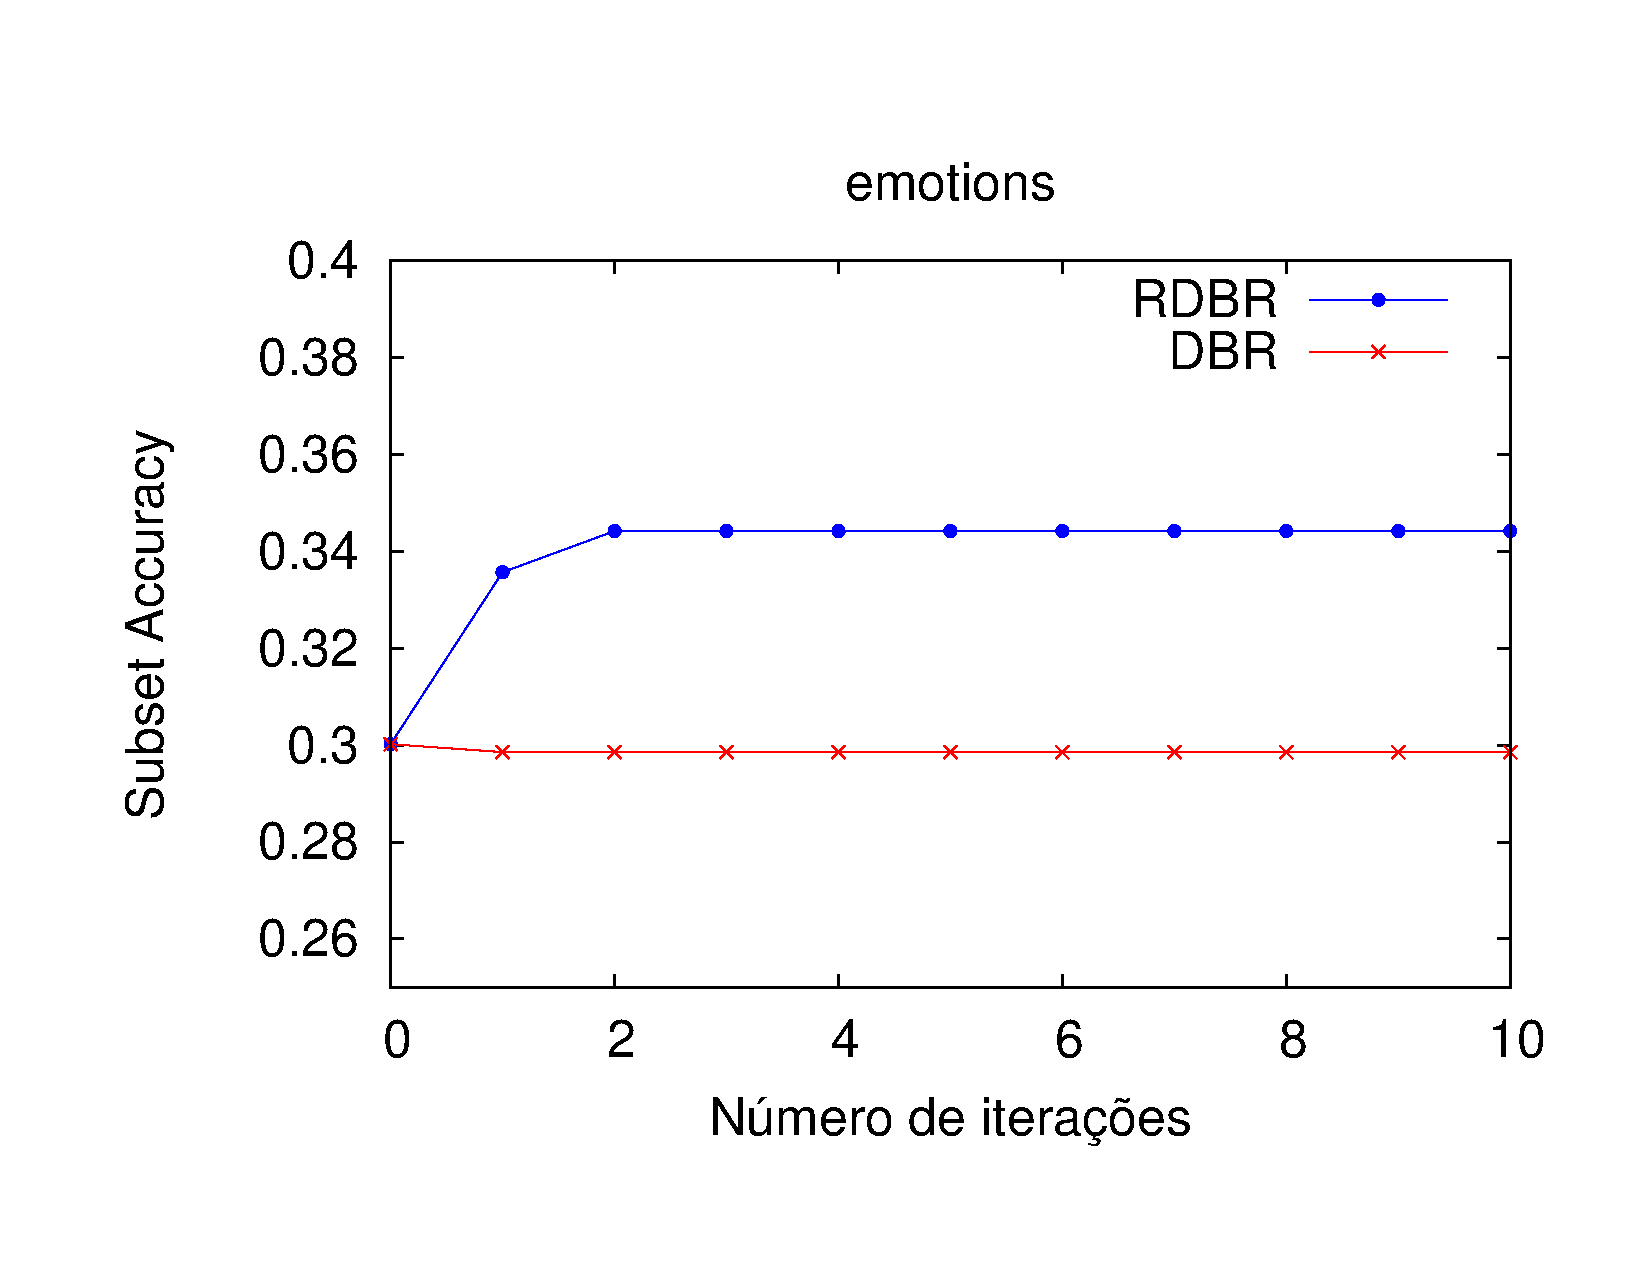
\includegraphics[angle=-90, width=1\linewidth]{plots/emotions}
  \caption{Emotions}
  \label{fig:subemotions}
\end{subfigure}%
\begin{subfigure}{.5\textwidth}
  \centering
  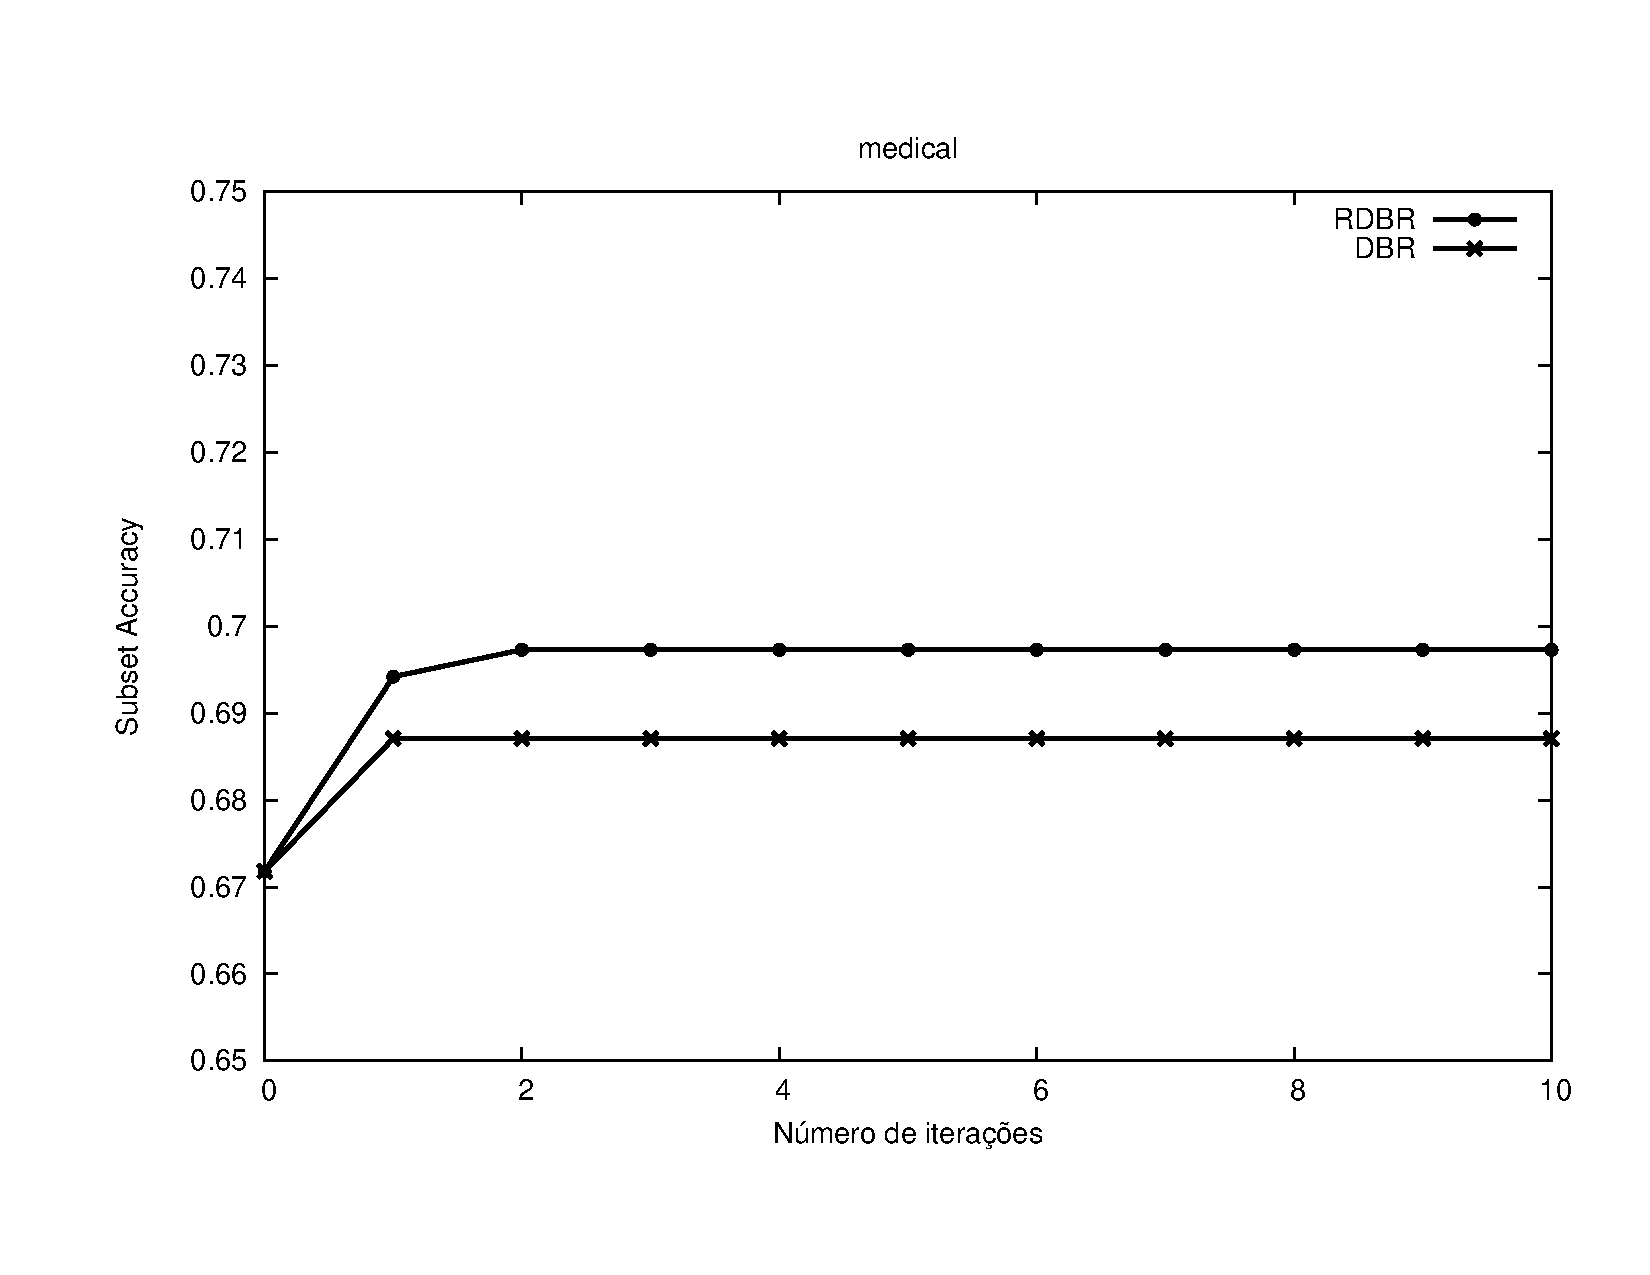
\includegraphics[angle=-90, width=1\linewidth]{plots/medical}
  \caption{Medical}
  \label{fig:submedical}
\end{subfigure}

\begin{subfigure}{.5\textwidth}
  \centering
  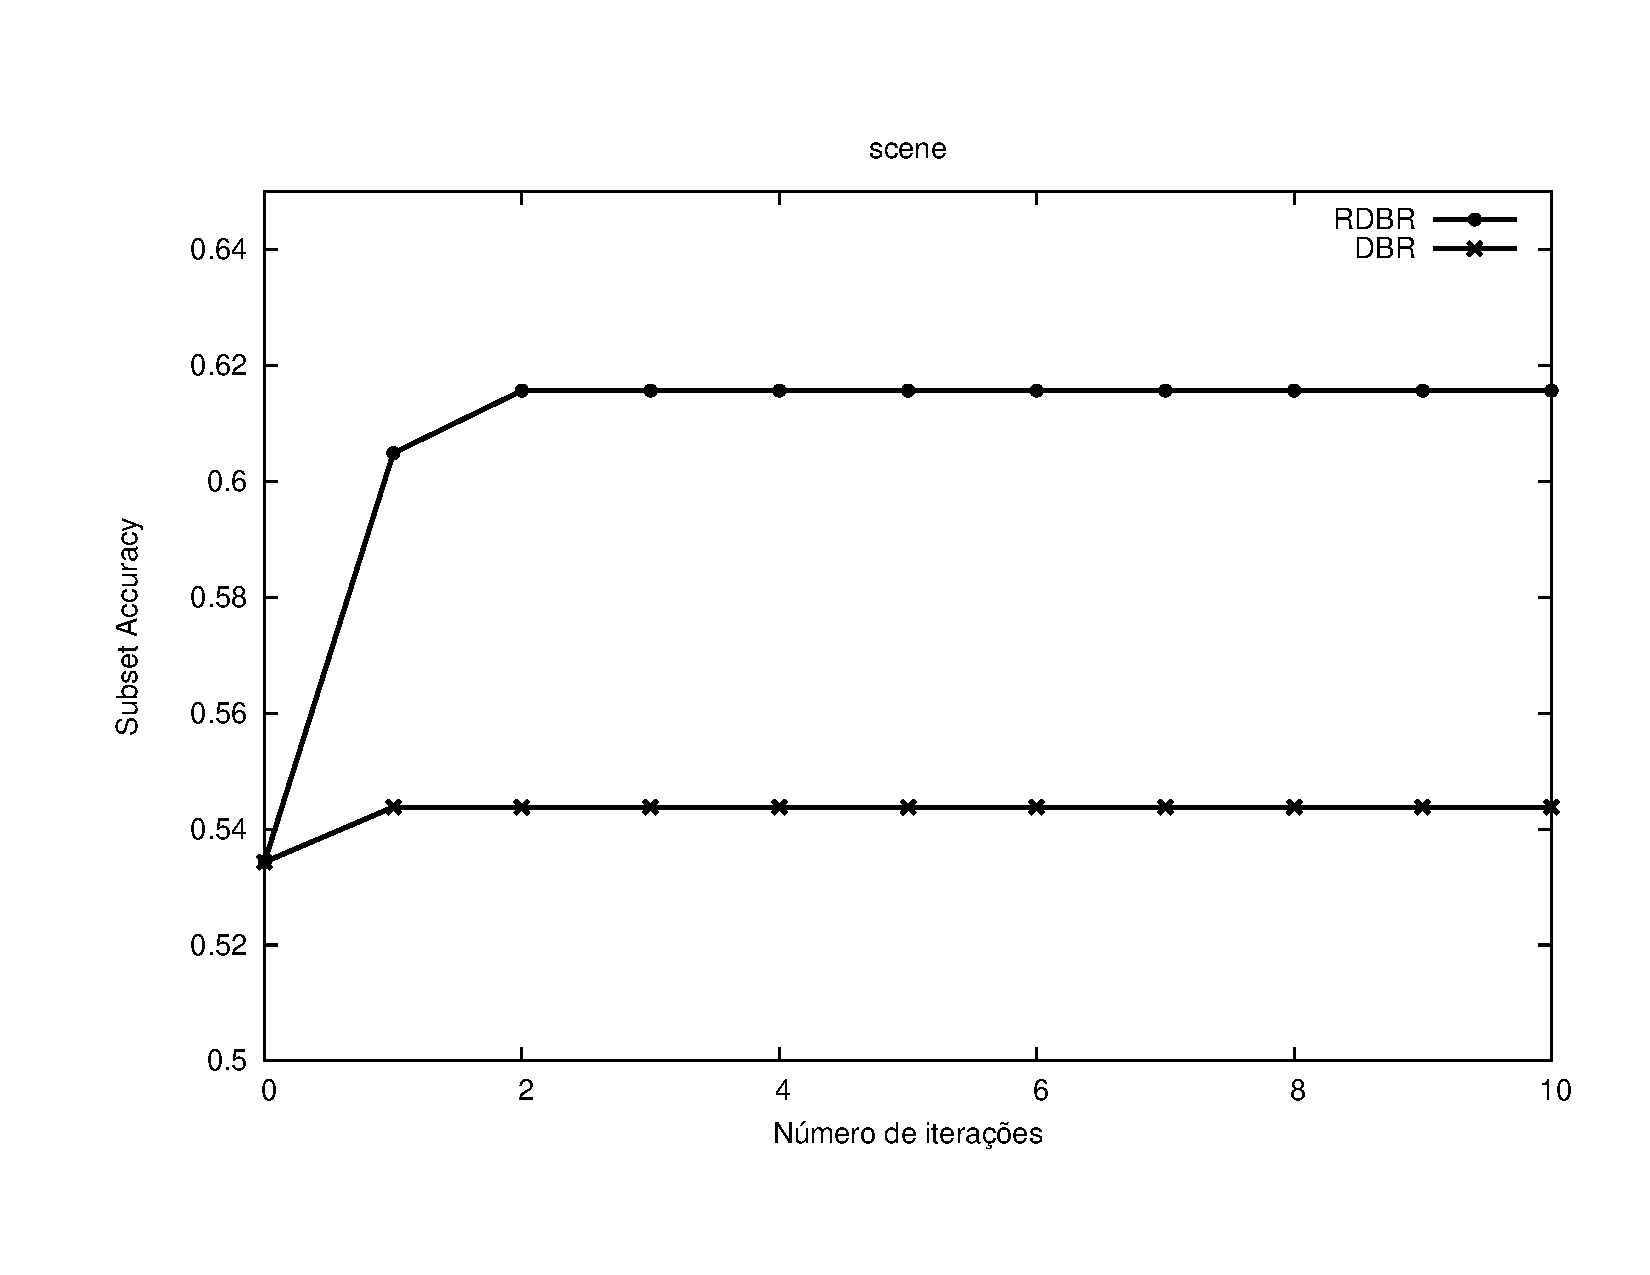
\includegraphics[angle=-90, width=1\linewidth]{plots/scene}
  \caption{Scene}
  \label{fig:subscene}
\end{subfigure}%
\begin{subfigure}{.5\textwidth}
  \centering
  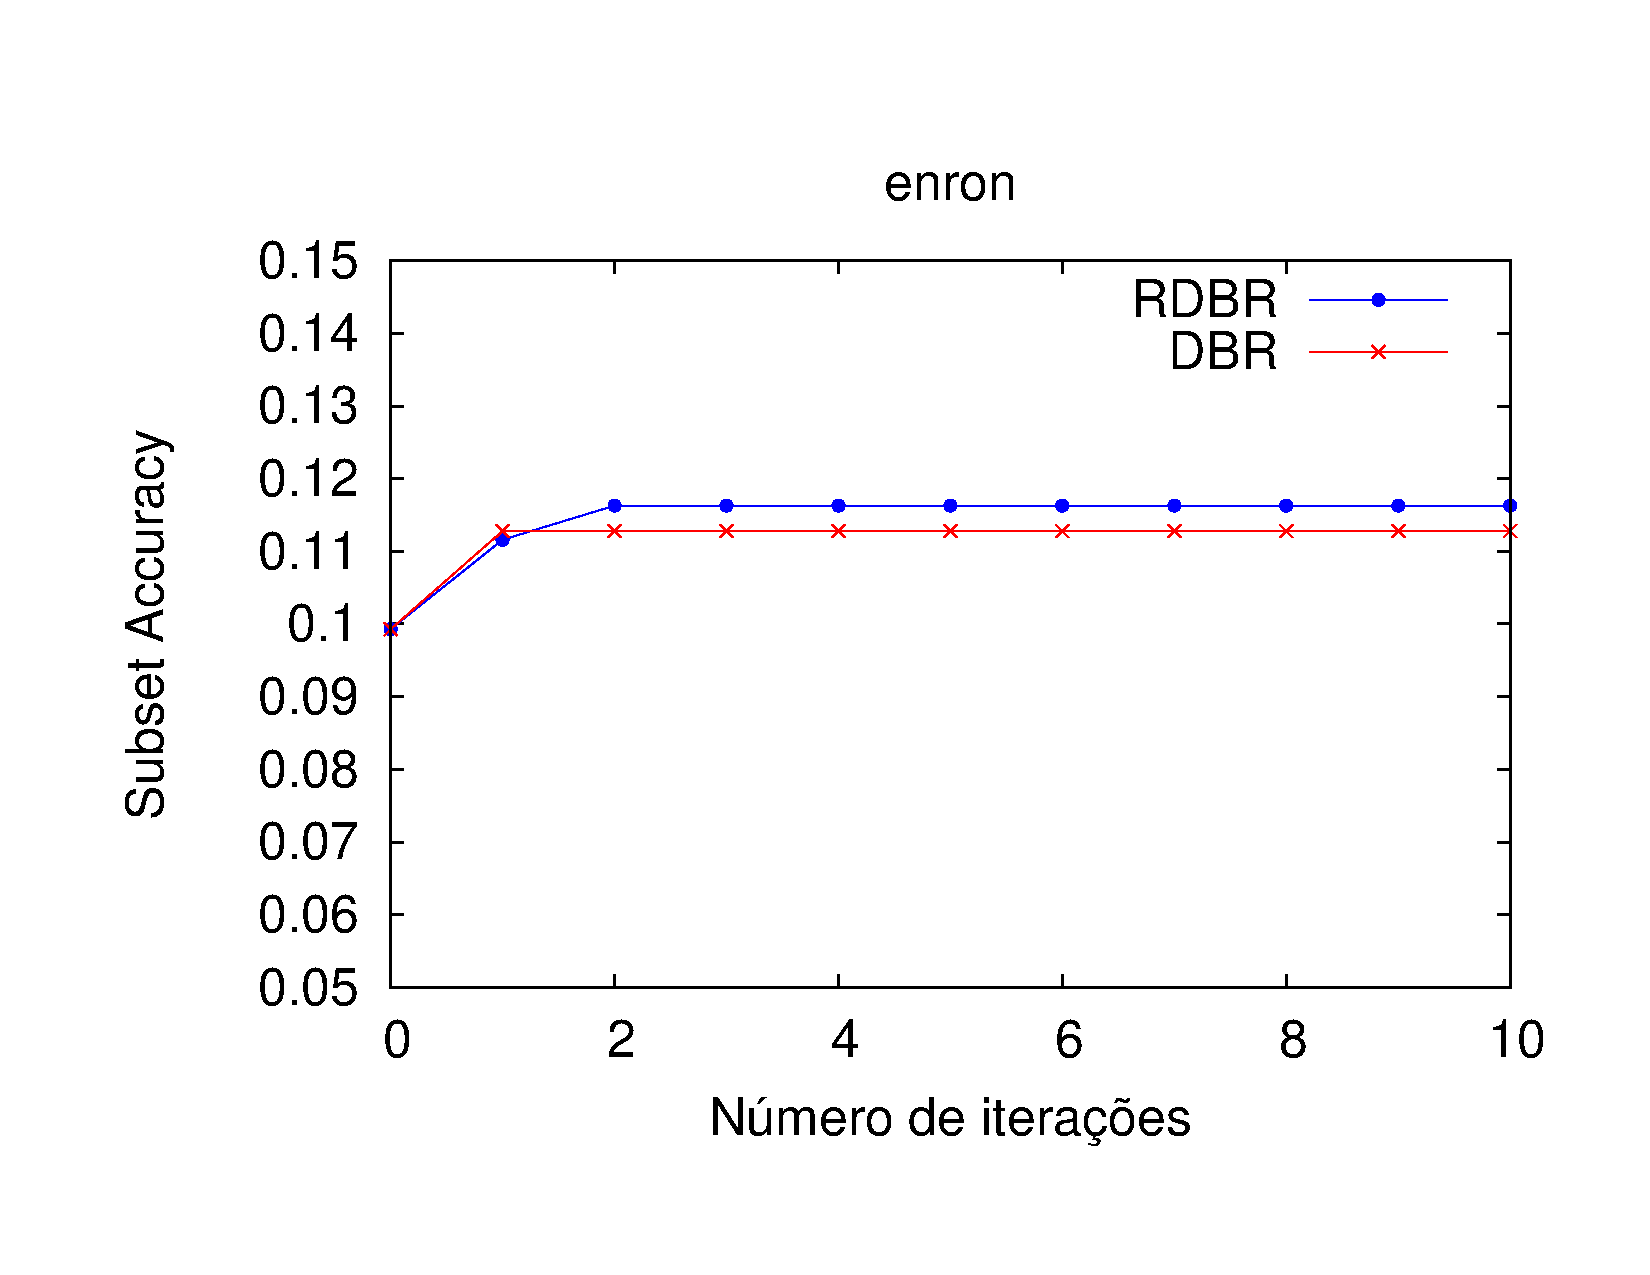
\includegraphics[angle=-90, width=1\linewidth]{plots/enron}
  \caption{Enron}
  \label{fig:subenron}
\end{subfigure}

\begin{subfigure}{.5\textwidth}
  \centering
  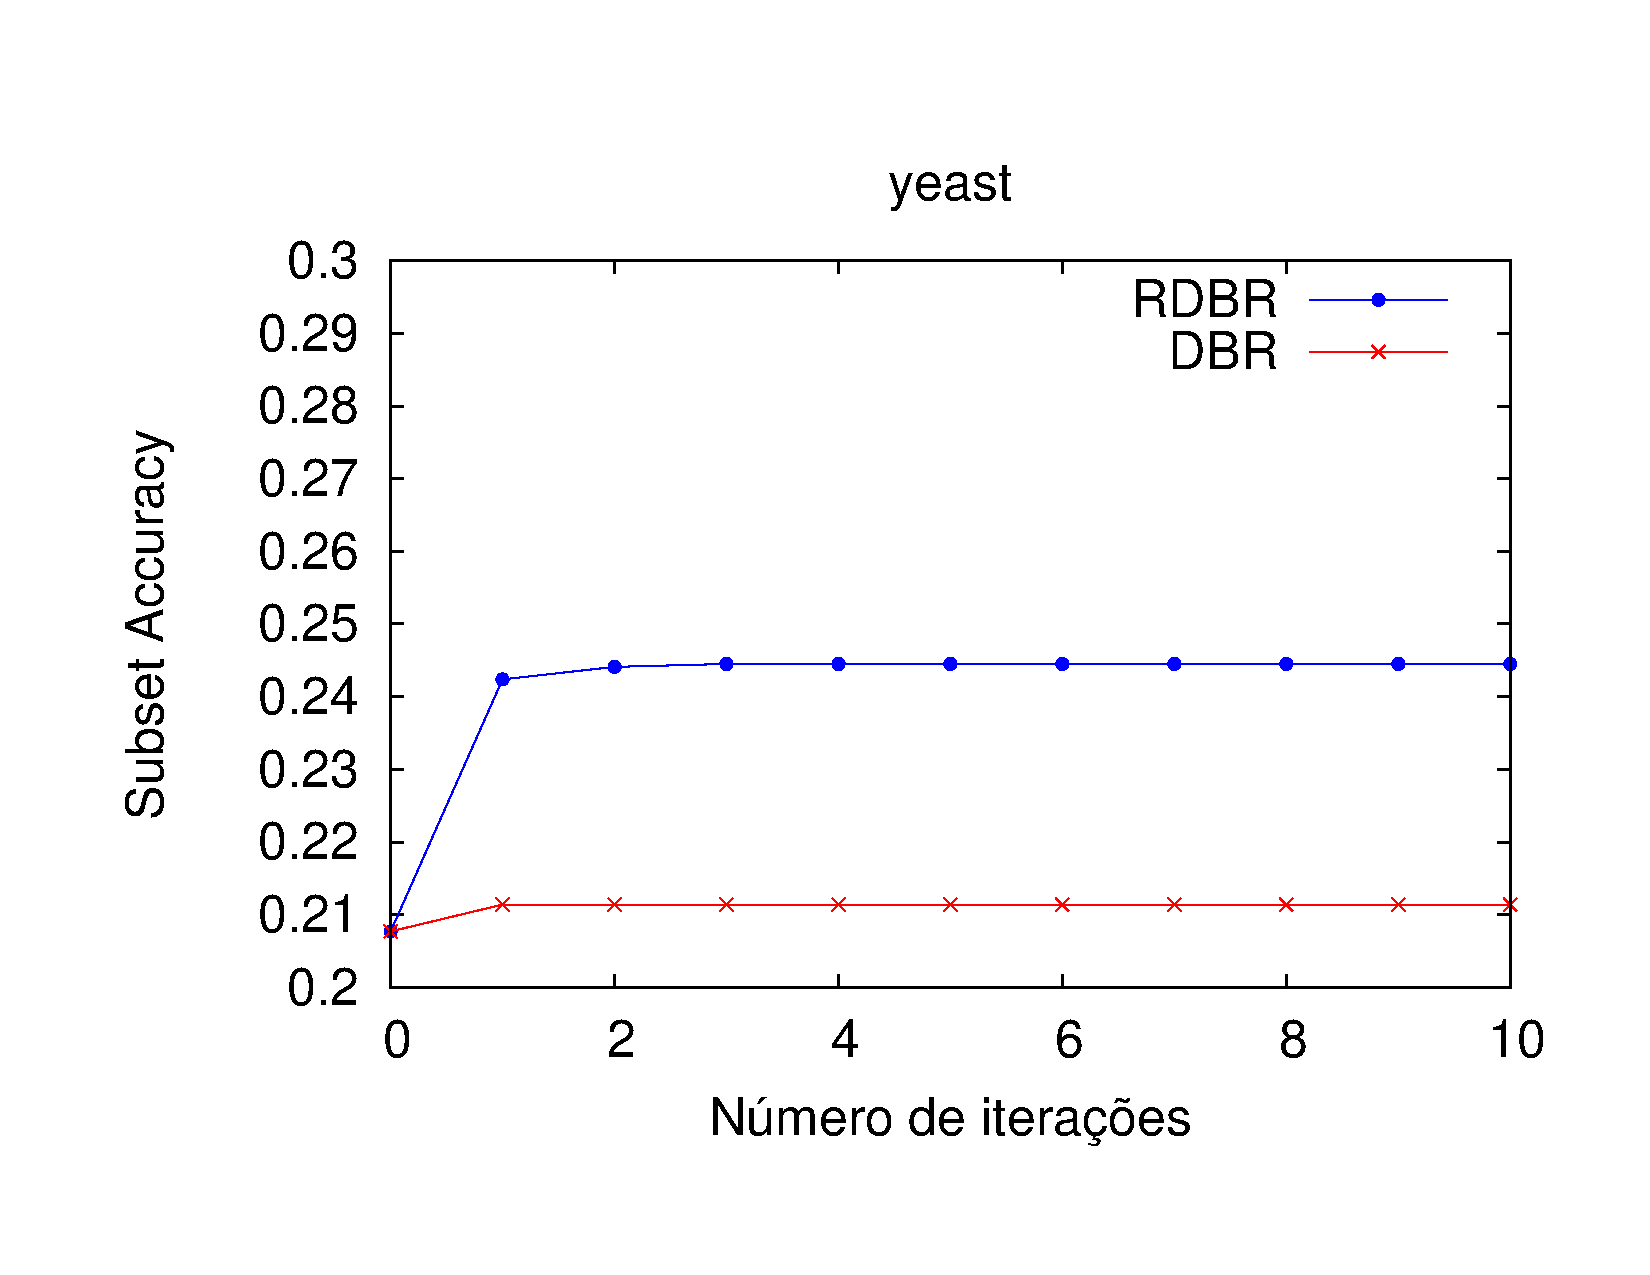
\includegraphics[angle=-90, width=1\linewidth]{plots/yeast}
  \caption{Yeast}
  \label{fig:subyeast}
\end{subfigure}
\caption{Gráficos de análise de desempenho do \MRLMa.}
\label{fig:test}
\end{figure}

\begin{figure}
\centering
 \begin{subfigure}{.5\textwidth}
  \centering
  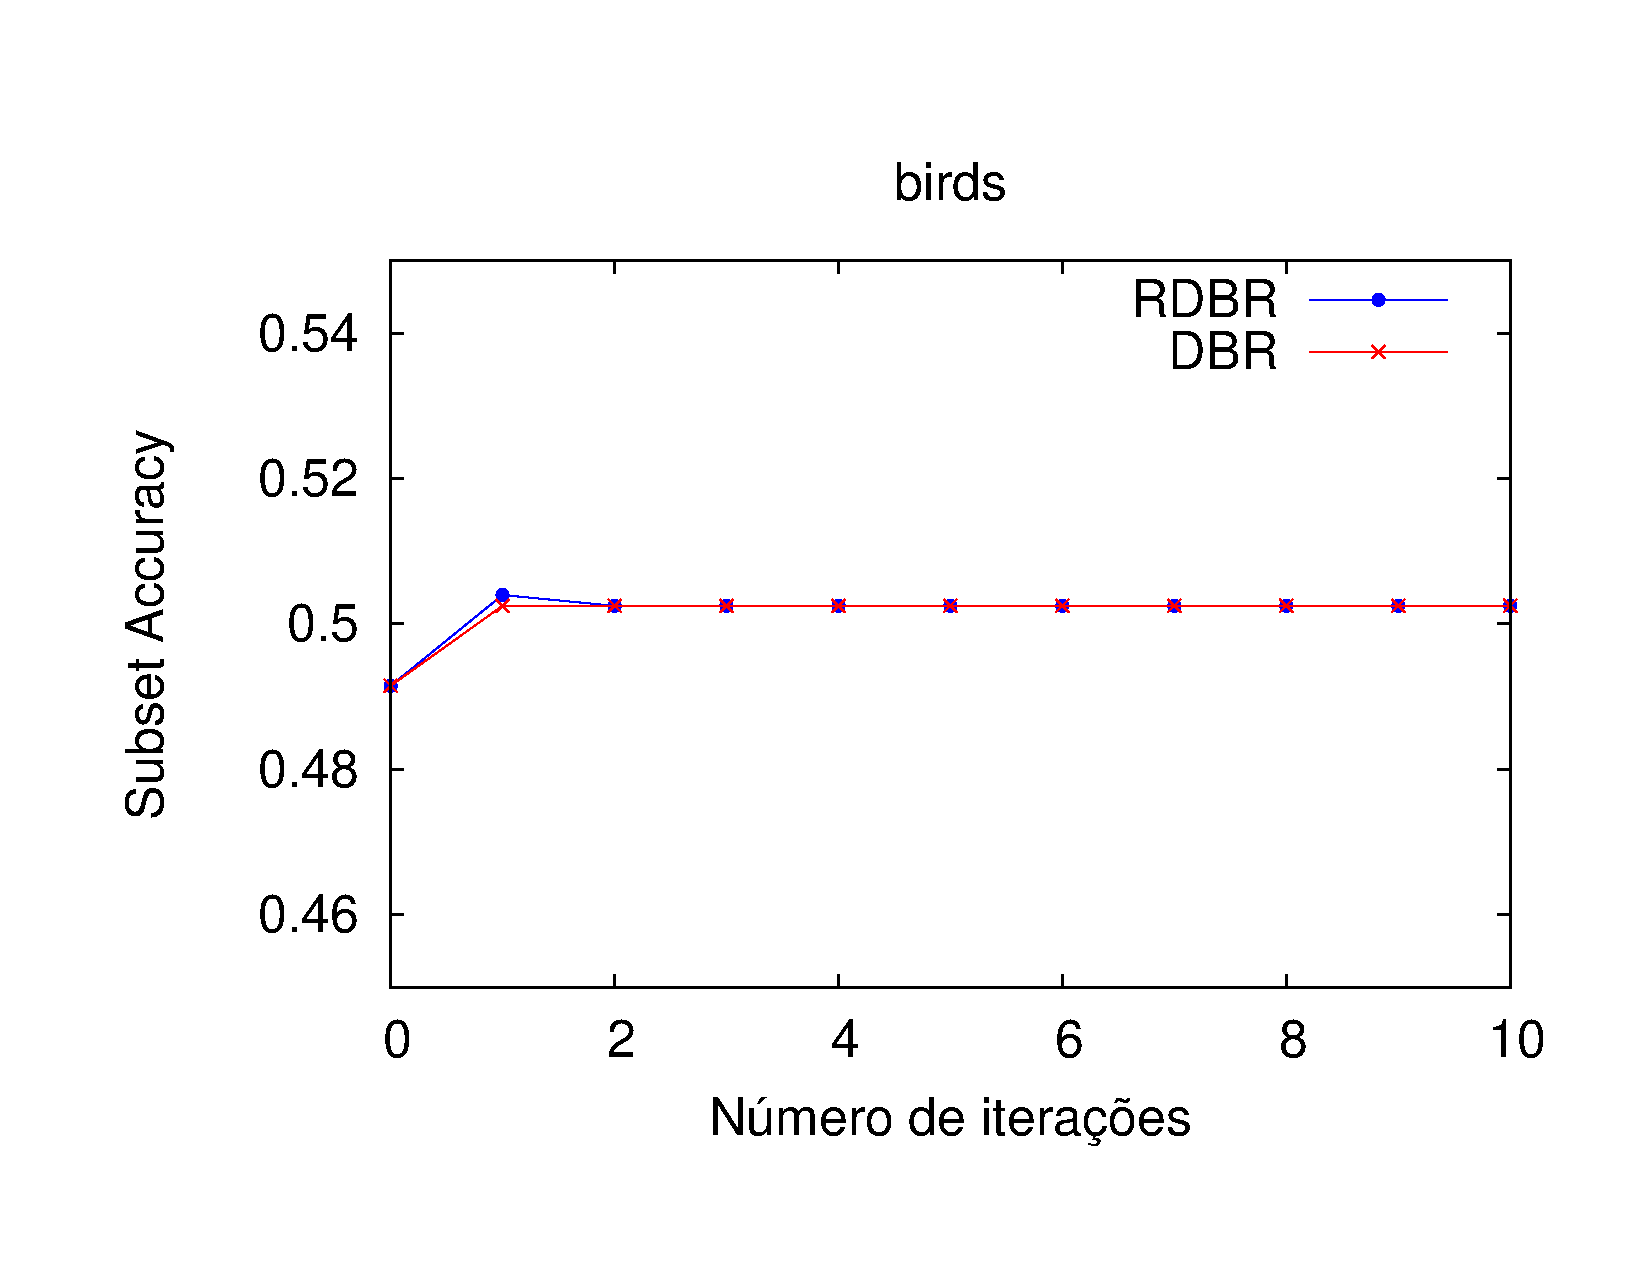
\includegraphics[angle=-90, width=1\linewidth]{plots/birds}
  \caption{Birds}
  \label{fig:subbirds}
\end{subfigure}%
\begin{subfigure}{.5\textwidth}
  \centering
  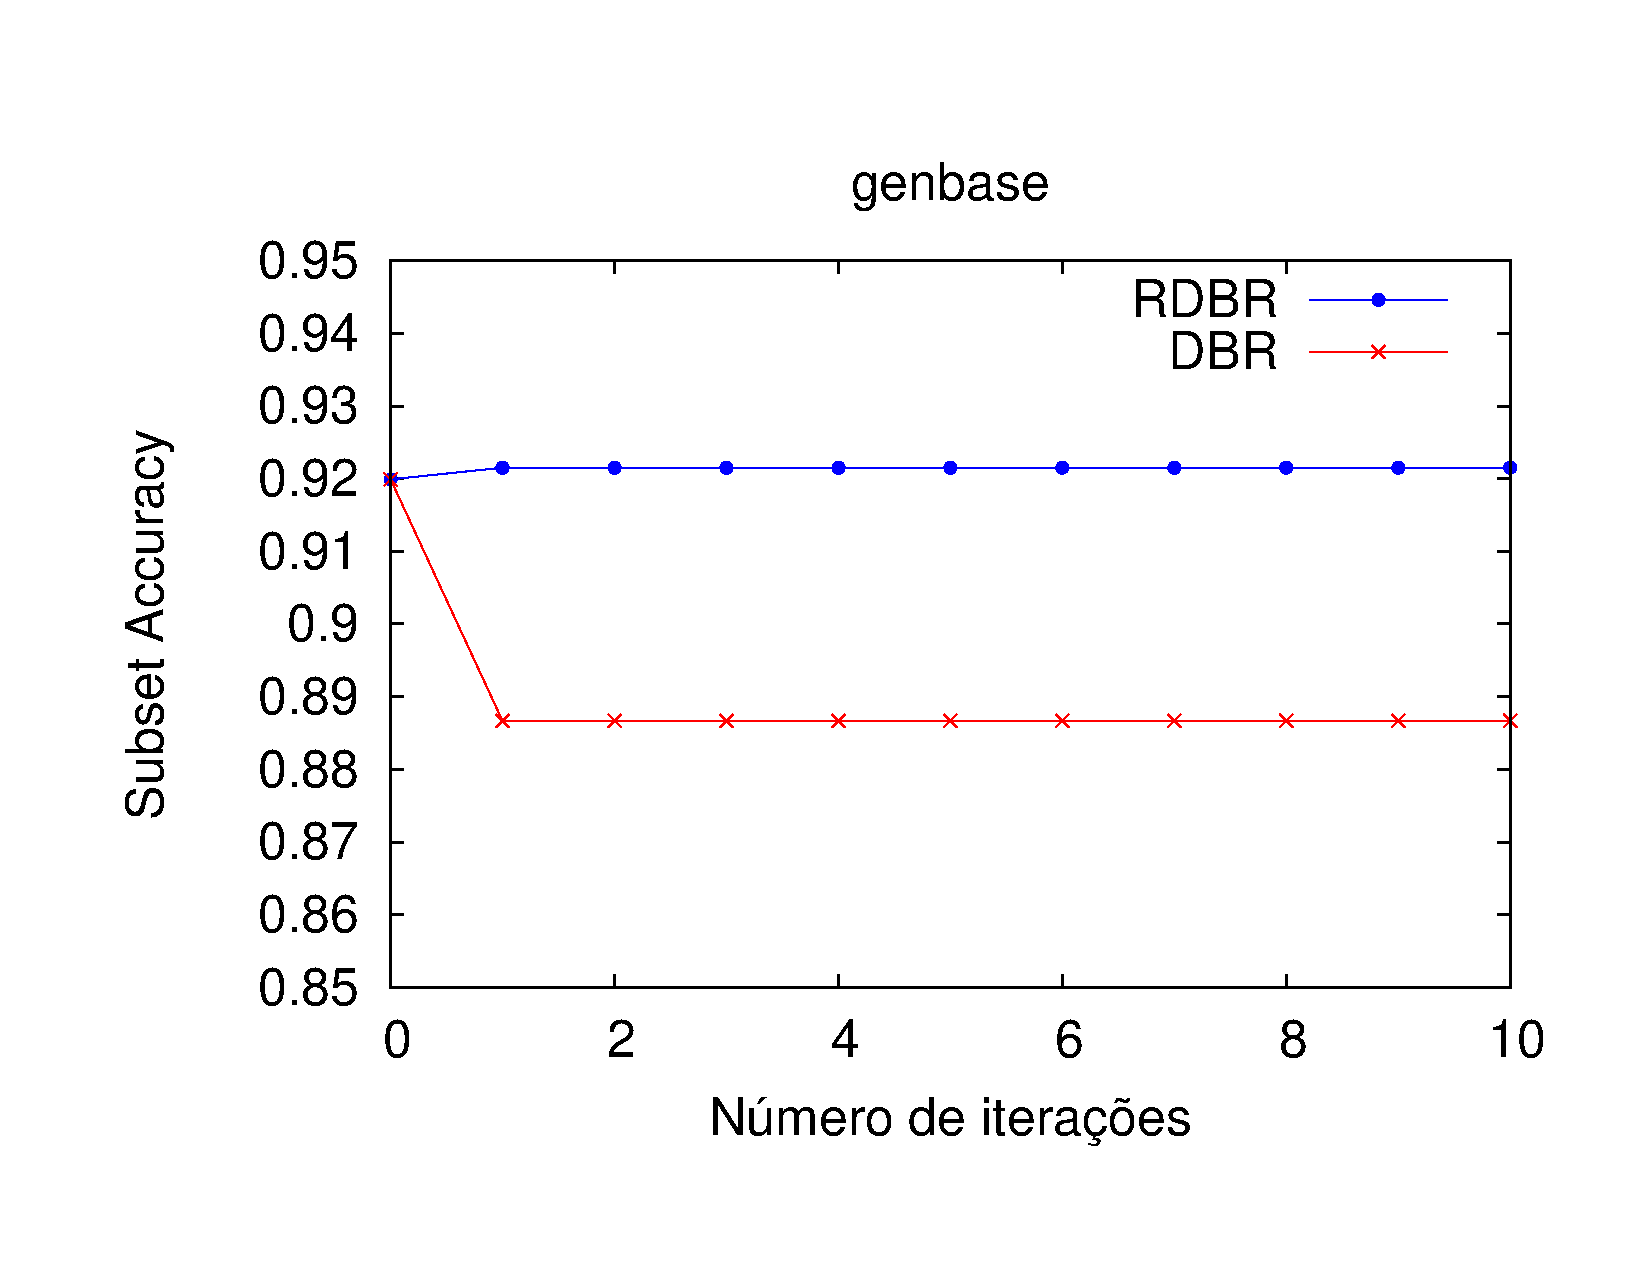
\includegraphics[angle=-90, width=1\linewidth]{plots/genbase}
  \caption{Genbase}
  \label{fig:subgenbase}
\end{subfigure}

\caption{Gráficos de análise de desempenho do \MRLMa~nos dois experimentos em que
o \MRLMa~não melhorou na sua segunda iteração.}
\end{figure}



É importante analisar o quanto o método aumenta o tamanho da base de dados uma vez que isso acarreta no aumento
do tempo de execução do algoritmo. Seja $r$ o número de rótulos, $n$ o número de instâncias de treino
e $m$ o número de atributos da base original, na fase de treinamento do \MRLMa, o número de base de dados utilizadas são
$2r$, cada uma contendo $n$ instâncias. Em metade delas, as instâncias contidas tem $m$ atributos e na outra metade $m+r$ atributos.
Já na fase de predição do algoritmo, no pior caso, o algoritmo usa $(k+1)r$ bases de dados de $n$ instâncias onde na primeira base, o
número de atributos é igual a $m$ e nas restantes é igual $m+r$. Vale ressaltar que nem todas essas bases de dados precisam ser
armazenados explicitamente na mémoria em espaços diferentes, algumas podem são reutilizadas no processo de predição.

% Em relação a complexidade algorítma do \MRLMa, ela pode ser
% aproximada pelo número de atributos destinados ao classificador base, uma vez que é um método de transformação
% e a maior parte do custo computacional se encontra no classificador base.
% A complexidade 




\chapter{Avaliação e Análise Experimental}
Neste capítulo é descrito as bases de dados multirrótulo usadas nos experimentos, as medidas de avaliação escolhidas e a escolha
dos parâmetros dos classificadores. 
A comparação e estudo dos métodos é feita considerando o custo computacional e a qualidade de predição.
A qualidade de predição é estimada pelo método de avaliação por validação cruzada \ref{sec:modelav} com 10 grupos
(\textit{10-fold cross-validation}) sobre \Nbases~bases de dados, todas apresentadas e descritas na subseção \ref{sec:datas}.

Para quantificar a qualidade de predição, 3 métricas foram utilizadas. As métricas escolhidas, bem como o motivo das escolhas,
são listadas:
\begin{itemize}
 \item Subset Accuracy, pois é mostrado que captura bem a correlação entre rótulos;
 \item Hamming Loss, pois é bem mais sensível que o Subset Accuracy;
 \item Example Based Accuracy, é o meio termo entre o Hamming Loss e o Subset Accuracy.
%  \item Tempo computacional, pois é @@@ etc...
\end{itemize}

As fórmulas para o cálculo de cada uma das métricas são apresentadas na seção \ref{sec:metrics}.
É interessante mostrar os resultados experimentais usando diferentes métricas, pois cada uma captura
um aspecto diferente da classificação. 

A análise experimental dos métodos se encontram divididos em dois estudos. O primeiro estudo consiste em
comparar os métodos quando todos usam o mesmo classificador base e o segundo em comparar cada combinação de um
modelo de classificação multirrótulo com uma configuração de parâmetros definida. 
O primeiro estudo tem por objetivo analisar se cada método multirrótulo apresentada desempenhos diferentes para
diferentes classificadores, ou seja, se o \textit{ranking} é alterado ao alterar o classificador base.
O segundo estudo tem por objetivo analisar os métodos de uma forma geral, uma vez que é desconhecido
o classificador base que melhor se adapta a cada base, a priori.

Num total, foram utilizados \Nml~modelos de classificação multirrótulos: BR, DBR, RDBR, CC, ECC e MCC.
Para cada um deles utilizou-se os seguintes classificadores base: KNN, SVM, \jqo e Regressão Logística \cite{classificadoresbases}. 
% Para o melhor entendimento, neste capítulo um método multirrótulo é definido como sendo a combinação
% de um modelo de classificação multirrótulo com uma configuração de parâmetros pré-definida. Assim, por exemplo,
% o classificador BR com KNN é considerado um método diferente do classificador BR com SVM.
% Isso, por um lado é bom
% pois testa o desempenho dos classificadores multirrótulo quando não é gasto tempo computacional para ajustar parâmetros.
% Por outro lado é ruim uma vez que considera os mesmos modelos de classificação como sendo completamente diferentes.
% Dessa forma, foram considerados 24 métodos multirrótulos e comparados entre si de forma experimental.


\section{Base de dados}
\label{sec:datas}
Todas as 7 bases de dados utilizadas nos experimentos foram obtidas de repositórios públicos pelo seguinte endereço virtual ??.
As bases de dados são apresentadas a seguir:

\begin{itemize}
\item \bf{Emotions}: ??
\item \bf{Scene}: ??
\item \bf{Yeast}: ??
\item \bf{Birds}: ??
\item \bf{Genbase}: ??
\item \bf{Medical}: ??
\item \bf{Enron}: ??	

\end{itemize}

\begin{table}[h]
\begin{tabular}{|c|ccccccc|}
\hline
% \textbf{}         & \textbf{}        & \textbf{}         & \multicolumn{2}{c}{\textbf{ATRIBUTOS}} & \textbf{}        & \textbf{}              & \textbf{}          \\
\textbf{BASE}     & \textbf{DOMÍNIO} & \textbf{EXEMPLOS} & \textbf{DIS} & \textbf{NUM} & \textbf{RÓTULOS} & \textbf{CARD} & \textbf{DENS} \\ \hline
\textbf{Emotions} & Música           & 593               & 0                 & 72                 & 6                & 1.869                  & 0.311              \\
\textbf{Scene}    & Imagem           & 2407              & 0                 & 294                & 6                & 1.074                  & 0.179              \\
\textbf{Yeast}    & Biologia         & 2417              & 0                 & 103                & 14               & 4.237                  & 0.303              \\
\textbf{Birds}    & Audio            & 645               & 2                 & 258                & 19               & 1.014                  & 0.053              \\
\textbf{Genbase}  & Biologia         & 662               & 1186              & 0                  & 27               & 1.252                  & 0.046              \\
\textbf{Medical}  & Texto            & 978               & 1449              & 0                  & 45               & 1.245                  & 0.028              \\
\textbf{Enron}    & Texto            & 1702              & 1001              & 0                  & 53               & 3.378                  & 0.064             \\ \hline
\end{tabular}
\caption{Resumo das bases de dados multirrótulos}
\label{tab:datas}
\end{table}

A tabela \ref{tab:datas} apresenta algumas estatísticas das bases de dados adquiridas.
Nela são apresentadas as seguintes informações de cada base de dados:
\begin{itemize}
  \item \textit{DIS}: número de atributos discretos;
  \item \textit{NUM}: número de atributos numéricos;
  \item \textit{CARD}: cardinalidade de rótulos na base de dados;
  \item \textit{DENS}: densidade de rótulos na base de dados.
\end{itemize}


% \section{Método de Comparação}
% \label{sec:methodcomp}


% 
% Este capítulo se encontra dividido em duas seções, na primeira foram analisados os
% resultados dos métodos de transformação para cada classificador base.
% Já na segunda seção cada combinação de método multirrótulo com classificador base foi considerado
% um método de transformação e seus resultados são comparados entre si juntamente com os métodos multirrótulos
% de adaptação.


\section{Resultados Experimentais}
\label{sec:exps}
Nesta seção é feita uma análise do desempenho dos métodos multirrótulos em cada uma das bases de dados
em diferentes métricas.
Essa seção é dividida em 4 subseções, uma para cada classificador base escolhido. Em cada uma
delas os métodos tiveram seus classificadores bases fixados.
A razão disso vem do fato de que queremos comparar os métodos multirrótulos entre si, e não os seus classificadores
bases.
Ao fixarmos o classificador base, 
o desempenho irá depender apenas do modelo de classificação multirrótulo
de cada um.
Em cada subseção e para cada métrica escolhida é apresentado uma tabela
contendo os valores da métrica para cada um dos métodos multirrótulo e
o ranking dos métodos multirrótulos. Conclusões e análises finais sobre
os fatos e observações levantados nessas subseções serão
dadas no capítulo \ref{sec:conclusions}.

% \subsection{Hammin}

% \begin{table}[h]
% \label{tab:hammingloss}
% 
% \caption{EXEMPLO DE TABELA, NAO É DE VERDADE AINDA!}
% 
% \end{table}

\subsection{KNN}
\begin{table}[h]
\begin{tabular}{lllllll}
\hline
\textbf{Dataset}    & \textbf{BR} & \textbf{CC} & \textbf{DBR} & \textbf{ECC} & \textbf{MCC} & \textbf{RDBR} \\ \hline
\textbf{Birds}      & 0.5084(3)   & 0.5007(5)   & 0.5116(1)    & 0.4991(6)    & 0.5023(4)    & 0.5115(2)     \\
\textbf{Emotions}   & 0.3101(5)   & 0.3406(1)   & 0.3119(4)    & 0.3(6)       & 0.3287(3)    & 0.3355(2)     \\
\textbf{Enron}      & 0.0717(5)   & 0.0899(3)   & 0.1005(2)    & 0.077(4)     & 0.0664(6)    & 0.1022(1)     \\
\textbf{Genbase}    & 0.9351(4)   & 0.9411(1)   & 0.9396(2)    & 0.0(6)       & 0.9336(5)    & 0.9381(3)     \\
\textbf{Medical}    & 0.4519(6)   & 0.503(2)    & 0.5(3)       & 0.4796(5)    & 0.4847(4)    & 0.5133(1)     \\
\textbf{Motorpump}  & 0.2857(1)   & 0.2799(4)   & 0.266(6)     & 0.2821(2)    & 0.2806(3)    & 0.2791(5)     \\
\textbf{Scene}      & 0.6452(6)   & 0.668(3)    & 0.6498(5)    & 0.661(4)     & 0.6788(2)    & 0.7009(1)     \\
\textbf{Yeast}      & 0.2209(6)   & 0.2454(3)   & 0.2226(5)    & 0.2301(4)    & 0.2615(1)    & 0.247(2)      \\ \hline
\textbf{Rank médio} & 4.5         & 2.75        & 3.5          & 4.625        & 3.5          & 2.125         \\ \hline
\end{tabular}
\caption{\legendaTab{Subset Accuracy}{KNN}}
\label{tab:SAknn}
\end{table}
\begin{table}[h]
\begin{tabular}{lllllll}
\hline
\textbf{Dataset}    & \textbf{BR} & \textbf{CC} & \textbf{DBR} & \textbf{ECC} & \textbf{MCC} & \textbf{RDBR} \\ \hline
\textbf{Birds}      & 0.0453(1)   & 0.0489(6)   & 0.0476(5)    & 0.0463(2)    & 0.0474(4)    & 0.0469(3)     \\
\textbf{Emotions}   & 0.1937(1)   & 0.2041(3)   & 0.2159(6)    & 0.1973(2)    & 0.2063(4)    & 0.2068(5)     \\
\textbf{Enron}      & 0.0581(1.5) & 0.059(3.5)  & 0.0606(5)    & 0.0581(1.5)  & 0.059(3.5)   & 0.0607(6)     \\
\textbf{Genbase}    & 0.0031(1)   & 0.0033(2)   & 0.0059(5)    & 1.0(6)       & 0.0038(4)    & 0.0034(3)     \\
\textbf{Medical}    & 0.0175(3.5) & 0.0165(1)   & 0.0188(5)    & 0.0171(2)    & 0.0175(3.5)  & 0.0189(6)     \\
\textbf{Motorpump}  & 0.1618(2)   & 0.1697(3)   & 0.1864(6)    & 0.161(1)     & 0.1714(5)    & 0.171(4)      \\
\textbf{Scene}      & 0.0925(2)   & 0.1003(5)   & 0.1065(6)    & 0.0931(3)    & 0.0965(4)    & 0.0906(1)     \\
\textbf{Yeast}      & 0.1981(2)   & 0.2159(6)   & 0.2109(5)    & 0.195(1)     & 0.2054(4)    & 0.2031(3)     \\ \hline
\textbf{Rank médio} & 1.75        & 3.6875      & 5.375        & 2.3125       & 4            & 3.875         \\ \hline
\end{tabular}
\caption{\legendaTab{Hamming Loss}{KNN}}
\label{tab:HLknn}
\end{table}
\begin{table}[h]
\begin{tabular}{lllllll}
\hline
\textbf{Dataset}    & \textbf{BR} & \textbf{CC} & \textbf{DBR} & \textbf{ECC} & \textbf{MCC} & \textbf{RDBR} \\ \hline
\textbf{Birds}      & 0.58(1)     & 0.5689(2)   & 0.5656(3)    & 0.5555(6)    & 0.5648(5)    & 0.5651(4)     \\
\textbf{Emotions}   & 0.5515(5)   & 0.5765(1)   & 0.5737(2)    & 0.545(6)     & 0.5604(4)    & 0.5691(3)     \\
\textbf{Enron}      & 0.2344(4)   & 0.2456(3)   & 0.264(2)     & 0.2198(5)    & 0.2085(6)    & 0.265(1)      \\
\textbf{Genbase}    & 0.9601(4)   & 0.9639(1)   & 0.9628(2)    & 0.0(6)       & 0.96(5)      & 0.9621(3)     \\
\textbf{Medical}    & 0.5147(6)   & 0.5724(3)   & 0.5966(1)    & 0.5455(5)    & 0.5476(4)    & 0.5857(2)     \\
\textbf{Motorpump}  & 0.5452(1)   & 0.5359(2)   & 0.5123(6)    & 0.5346(3)    & 0.5289(4)    & 0.5245(5)     \\
\textbf{Scene}      & 0.6742(6)   & 0.6987(4)   & 0.7123(2)    & 0.692(5)     & 0.7089(3)    & 0.7322(1)     \\
\textbf{Yeast}      & 0.524(4)    & 0.52(6)     & 0.5238(5)    & 0.5361(2)    & 0.5368(1)    & 0.5343(3)     \\ \hline
\textbf{Rank médio} & 3.875       & 2.75        & 2.875        & 4.75         & 4            & 2.75          \\ \hline
\end{tabular}
\caption{\legendaTab{\EBA}{KNN}}
\label{tab:EBAknn}
\end{table}


Vejamos alguns pontos interessantes nos testes das tabelas
\ref{tab:SAknn},\ref{tab:HLknn} e \ref{tab:EBAknn}.
Note que o \textit{ranking} dos métodos mudou bastante de métrica para métrica.
No caso do BR, o ranking médio caiu de $4.5$ no \SA para $1.75$ no Hamming Loss, ou seja,
de penúltimo colocado no ranking médio para o primeiro colocado. 
Lembre-se de que cada métrica captura um aspecto diferente do método.
Note que para a base de dados \textit{Enron}, o valor do \SA~é o mais baixo dentre todas bases.
Isso é esperado uma vez que é a base \textit{Enron} é a base com maior número de rótulos ($53$) e o \SA
exige fortemente que a predição do classificador acerte a única possível combinação dentre as $2^{53}$ possíveis.
Mas o interessante é que, apesar do \SA~ser o pior para essa base, o \HL~é o quarto melhor.
Isso sugere que há um alguns poucos rótulos que são difíceis de serem corretamente preditos.

Para o classificador base KNN, o RDBR obteve o melhor resultado na métrica \SA~e na métrica \EBA.


\subsection{SVM}
\begin{table}[h]
\begin{tabular}{lllllll}
\hline
\textbf{Dataset} & \textbf{BR} & \textbf{CC} & \textbf{DBR} & \textbf{ECC} & \textbf{MCC} & \textbf{RDBR} \\ \hline
\textbf{Birds}           & 0.4775(2)   & 0.4496(6)   & 0.4528(4)    & 0.4604(3)    & 0.4822(1)    & 0.4527(5)     \\
\textbf{Emotions}        & 0.2917(6)   & 0.3051(5)   & 0.3086(4)    & 0.3356(2)    & 0.3255(3)    & 0.3558(1)     \\
\textbf{Enron}           & 0.0741(6)   & 0.1052(4)   & 0.094(5)     & 0.1334(1)    & 0.1087(2)    & 0.1075(3)     \\
\textbf{Genbase}         & 0.9033(5)   & 0.9154(1)   & 0.9123(3)    & 0.8836(6)    & 0.9047(4)    & 0.9139(2)     \\
\textbf{Medical}         & 0.5931(6)   & 0.6228(4.5) & 0.6228(4.5)  & 0.6483(1)    & 0.6361(3)    & 0.6443(2)     \\
\textbf{Motorpump}       & 0.2186(6)   & 0.2755(3)   & 0.2558(5)    & 0.293(1)     & 0.2748(4)    & 0.2763(2)     \\
\textbf{Scene}           & 0.5322(6)   & 0.6394(3)   & 0.5422(5)    & 0.6572(1)    & 0.6548(2)    & 0.614(4)      \\
\textbf{Yeast}           & 0.1489(6)   & 0.1965(3)   & 0.1535(5)    & 0.2006(2)    & 0.2193(1)    & 0.1845(4)     \\ \hline
\textbf{Rank médio}      & 5.375       & 3.6875      & 4.4375       & 2.125        & 2.5          & 2.875         \\ \hline
\end{tabular}
\caption{\legendaTab{Subset Accuracy}{SVM}}
\label{tab:SAsvm}
\end{table}
\begin{table}[h]
\begin{tabular}{lllllll}
\hline
\textbf{Dataset}    & \textbf{BR} & \textbf{CC} & \textbf{DBR} & \textbf{ECC} & \textbf{MCC} & \textbf{RDBR} \\ \hline
\textbf{Birds}      & 0.0596(2)   & 0.0651(4)   & 0.0662(6)    & 0.0567(1)    & 0.0624(3)    & 0.066(5)      \\
\textbf{Emotions}   & 0.1917(2)   & 0.2134(5)   & 0.2156(6)    & 0.1847(1)    & 0.2108(4)    & 0.1929(3)     \\
\textbf{Enron}      & 0.0799(6)   & 0.0744(3.5) & 0.0744(3.5)  & 0.0529(1)    & 0.0726(2)    & 0.0762(5)     \\
\textbf{Genbase}    & 0.0041(5)   & 0.0036(2)   & 0.0035(1)    & 0.0051(6)    & 0.004(4)     & 0.0037(3)     \\
\textbf{Medical}    & 0.0127(6)   & 0.0126(4.5) & 0.0125(2.5)  & 0.0112(1)    & 0.0125(2.5)  & 0.0126(4.5)   \\
\textbf{Motorpump}  & 0.1657(2)   & 0.167(4)    & 0.1701(6)    & 0.154(1)     & 0.1685(5)    & 0.1659(3)     \\
\textbf{Scene}      & 0.1066(3)   & 0.1067(4)   & 0.2094(6)    & 0.0903(1)    & 0.1029(2)    & 0.1167(5)     \\
\textbf{Yeast}      & 0.2001(1)   & 0.2246(6)   & 0.221(5)     & 0.2027(2)    & 0.2108(4)    & 0.2103(3)     \\ \hline
\textbf{Rank médio} & 3.375       & 4.125       & 4.5          & 1.75         & 3.3125       & 3.9375        \\ \hline
\end{tabular}
\caption{\legendaTab{Hamming Loss}{SVM}}
\label{tab:HLsvm}
\end{table}
\begin{table}[\tabmode]
\begin{tabular}{lllllll}
\hline
\textbf{Dataset}    & \textbf{BR} & \textbf{CC} & \textbf{DBR} & \textbf{ECC} & \textbf{MCC} & \textbf{RDBR} \\ \hline
\textbf{Birds}      & 0.6068(1)   & 0.586(4)    & 0.5786(6)    & 0.5975(3)    & 0.6041(2)    & 0.5828(5)     \\
\textbf{Emotions}   & 0.5345(6)   & 0.5434(5)   & 0.5842(2)    & 0.5781(3)    & 0.5541(4)    & 0.6018(1)     \\
\textbf{Enron}      & 0.3503(6)   & 0.3728(3)   & 0.3661(5)    & 0.4331(1)    & 0.382(2)     & 0.3688(4)     \\
\textbf{Genbase}    & 0.9552(5)   & 0.9608(1)   & 0.9603(2)    & 0.9444(6)    & 0.9555(4)    & 0.9597(3)     \\
\textbf{Medical}    & 0.6983(6)   & 0.713(4)    & 0.714(3)     & 0.7226(2)    & 0.7128(5)    & 0.727(1)      \\
\textbf{Motorpump}  & 0.465(6)    & 0.5275(5)   & 0.5488(2)    & 0.5535(1)    & 0.5286(4)    & 0.5398(3)     \\
\textbf{Scene}      & 0.6065(6)   & 0.6916(3)   & 0.6233(5)    & 0.7036(1)    & 0.7018(2)    & 0.6604(4)     \\
\textbf{Yeast}      & 0.5064(4)   & 0.4921(6)   & 0.4949(5)    & 0.5243(2)    & 0.5258(1)    & 0.5142(3)     \\ \hline
\textbf{Rank médio} & 5           & 3.875       & 3.75         & 2.375        & 3            & 3             \\ \hline
\end{tabular}
\caption{\legendaTab{\EBA}{SVM}}
\label{tab:EBAsvm}
\end{table}

Nas tabelas
\ref{tab:SAsvm},\ref{tab:HLsvm} e \ref{tab:EBAsvm} observamos os mesmo pontos
interessantes que nas tabelas do KNN, (\ref{tab:SAknn},\ref{tab:HLknn} e \ref{tab:EBAknn}):
O \textit{ranking} muda bastante de métrica para métrica e o \SA~é baixo para algumas base porém
o \HL~é bom para as mesmas. No entanto, o modelo de classificação multirrótulo que mais se adaptou ao SVM foi
o \ECC. Adicionalmente, a ordem dos métodos que obtiverem o melhor rank médio alterou-se consideravelmente.
Para o \SA~a ordem crescente era \MRLMa,MCC,DBR,CC,BR,ECC com o KNN, mas com o SVM a ordem mudou para ECC,MCC,\MRLMa,CC,DBR,BR.

\subsection{\jqo}
\begin{table}[h]
\begin{tabular}{lllllll}
\hline
\textbf{Dataset}    & \textbf{BR} & \textbf{CC} & \textbf{DBR} & \textbf{ECC} & \textbf{MCC} & \textbf{RDBR} \\ \hline
\textbf{Birds}      & 0.4683(6)   & 0.4791(4)   & 0.49(2.5)    & 0.5318(1)    & 0.4775(5)    & 0.49(2.5)     \\
\textbf{Emotions}   & 0.1637(6)   & 0.1888(4)   & 0.1822(5)    & 0.3002(1)    & 0.2328(2)    & 0.2244(3)     \\
\textbf{Enron}      & 0.1034(5)   & 0.1257(2)   & 0.0975(6)    & 0.1381(1)    & 0.114(3)     & 0.1116(4)     \\
\textbf{Genbase}    & 0.9714(2.5) & 0.9699(5)   & 0.9714(2.5)  & 0.9623(6)    & 0.9714(2.5)  & 0.9714(2.5)   \\
\textbf{Medical}    & 0.6718(6)   & 0.6902(4)   & 0.6974(2)    & 0.6739(5)    & 0.6932(3)    & 0.7035(1)     \\
\textbf{Motorpump}  & 0.2274(6)   & 0.2536(3)   & 0.2376(5)    & 0.3185(1)    & 0.2442(4)    & 0.2573(2)     \\
\textbf{Scene}      & 0.4408(5)   & 0.5692(2)   & 0.4366(6)    & 0.5962(1)    & 0.5501(3)    & 0.543(4)      \\
\textbf{Yeast}      & 0.0658(6)   & 0.1448(2)   & 0.0666(5)    & 0.1684(1)    & 0.1303(3)    & 0.1212(4)     \\ \hline
\textbf{Rank médio} & 5.3125      & 3.25        & 4.25         & 2.125        & 3.1875       & 2.875         \\ \hline
\end{tabular}
\caption{\legendaTab{Subset Accuracy}{\jqo}}
\label{tab:SAj48}
\end{table}
\begin{table}[h]
\begin{tabular}{lllllll}
\hline
\textbf{Dataset}    & \textbf{BR} & \textbf{CC} & \textbf{DBR} & \textbf{ECC} & \textbf{MCC} & \textbf{RDBR} \\ \hline
\textbf{Birds}      & 0.0517(5)   & 0.0501(2)   & 0.051(3.5)   & 0.0415(1)    & 0.052(6)     & 0.051(3.5)    \\
\textbf{Emotions}   & 0.2529(2)   & 0.2693(5)   & 0.2729(6)    & 0.1945(1)    & 0.2575(3)    & 0.2645(4)     \\
\textbf{Enron}      & 0.0509(2)   & 0.054(5)    & 0.0559(6)    & 0.049(1)     & 0.0532(3)    & 0.0537(4)     \\
\textbf{Genbase}    & 0.0012(2.5) & 0.0013(5)   & 0.0012(2.5)  & 0.0016(6)    & 0.0012(2.5)  & 0.0012(2.5)   \\
\textbf{Medical}    & 0.01(5)     & 0.0097(3.5) & 0.0093(1)    & 0.0101(6)    & 0.0097(3.5)  & 0.0095(2)     \\
\textbf{Motorpump}  & 0.1753(3)   & 0.174(2)    & 0.1791(6)    & 0.1398(1)    & 0.1769(4)    & 0.1782(5)     \\
\textbf{Scene}      & 0.1307(2)   & 0.1334(3)   & 0.1779(6)    & 0.0941(1)    & 0.1378(4)    & 0.1449(5)     \\
\textbf{Yeast}      & 0.2489(2)   & 0.268(4)    & 0.2829(6)    & 0.2046(1)    & 0.2702(5)    & 0.2637(3)     \\ \hline
\textbf{Rank médio} & 2.9375      & 3.6875      & 4.625        & 2.25         & 3.875        & 3.625         \\ \hline
\end{tabular}
\caption{\legendaTab{Hamming Loss}{\jqo}}
\label{tab:HLj48}
\end{table}
\begin{table}[\tabmode]
\begin{tabular}{lllllll}
\hline
\textbf{Dataset}    & \textbf{BR} & \textbf{CC} & \textbf{DBR} & \textbf{ECC} & \textbf{MCC} & \textbf{RDBR} \\ \hline
\textbf{Birds}      & 0.5628(6)   & 0.5706(4)   & 0.5764(3)    & 0.5935(1)    & 0.5629(5)    & 0.5777(2)     \\
\textbf{Emotions}   & 0.4447(4)   & 0.4405(5)   & 0.4176(6)    & 0.5238(1)    & 0.469(2)     & 0.4631(3)     \\
\textbf{Enron}      & 0.4131(4)   & 0.4115(5)   & 0.4141(3)    & 0.44(1)      & 0.3989(6)    & 0.4163(2)     \\
\textbf{Genbase}    & 0.9854(2.5) & 0.9847(5)   & 0.9854(2.5)  & 0.9779(6)    & 0.9854(2.5)  & 0.9854(2.5)   \\
\textbf{Medical}    & 0.7585(5)   & 0.7707(4)   & 0.7822(2)    & 0.7573(6)    & 0.7732(3)    & 0.7845(1)     \\
\textbf{Motorpump}  & 0.5252(6)   & 0.549(2)    & 0.5347(5)    & 0.6046(1)    & 0.5393(4)    & 0.5444(3)     \\
\textbf{Scene}      & 0.54(5)     & 0.6205(2)   & 0.5336(6)    & 0.6276(1)    & 0.6011(3)    & 0.5843(4)     \\
\textbf{Yeast}      & 0.4357(3)   & 0.4252(4)   & 0.4171(6)    & 0.4932(1)    & 0.4196(5)    & 0.4451(2)     \\ \hline
\textbf{Rank médio} & 4.4375      & 3.875       & 4.1875       & 2.25         & 3.8125       & 2.4375        \\ \hline
\end{tabular}
\caption{\legendaTab{\EBA}{\jqo}}
\label{tab:EBAj48}
\end{table}

Além de reforçar os mesmos pontos interessantes citados nos classificadores bases anteriores,
os testes com o \jqo, apresentados nas tabelas \ref{tab:SAj48},\ref{tab:HLj48} e \ref{tab:EBAj48}, mostraram mais uma vez que o \ECC~e o \MRLMa~obtiveram os melhores resultados, exceto
no Hamming Loss, na qual o BR superou o \MRLMa.

\subsection{Logi}
\begin{table}[h]
\begin{tabular}{lllllll}
\hline
\textbf{Subset Accuracy} & \textbf{BR} & \textbf{CC} & \textbf{DBR} & \textbf{ECC} & \textbf{MCC} & \textbf{RDBR} \\ \hline
\textbf{Birds}           & 0.4403(6)   & 0.4512(2)   & 0.4434(5)    & 0.4836(1)    & 0.448(3.5)   & 0.448(3.5)    \\
\textbf{Emotions}        & 0.2343(5)   & 0.268(1)    & 0.2073(6)    & 0.2561(2)    & 0.2411(4)    & 0.2427(3)     \\
\textbf{Enron}           & 0.1093(3)   & 0.1134(2)   & 0.1017(6)    & 0.1257(1)    & 0.1081(4)    & 0.107(5)      \\
\textbf{Genbase}         & 0.9562(4)   & 0.9532(5)   & 0.9577(2)    & 0.7901(6)    & 0.9577(2)    & 0.9577(2)     \\
\textbf{Medical}         & 0.4499(6)   & 0.4653(5)   & 0.4684(4)    & 0.5297(1)    & 0.4745(3)    & 0.4827(2)     \\
\textbf{Motorpump}       & 0.2857(6)   & 0.3003(3)   & 0.2944(5)    & 0.3039(1)    & 0.2995(4)    & 0.301(2)      \\
\textbf{Scene}           & 0.4989(5)   & 0.6003(2)   & 0.4944(6)    & 0.5941(3)    & 0.6061(1)    & 0.5845(4)     \\
\textbf{Yeast}           & 0.1369(6)   & 0.1841(2)   & 0.1386(5)    & 0.1709(3)    & 0.1907(1)    & 0.168(4)      \\ \hline
\textbf{Rank médio}      & 5.125       & 2.75        & 4.875        & 2.25         & 2.8125       & 3.1875        \\ \hline
\end{tabular}
\caption{\legendaTab{Subset Accuracy}{Regressão Logística}}
\label{tab:SAlogi}
\end{table}
\begin{table}[h]
\begin{tabular}{lllllll}
\hline
\textbf{Dataset}    & \textbf{BR} & \textbf{CC} & \textbf{DBR} & \textbf{ECC} & \textbf{MCC} & \textbf{RDBR} \\ \hline
\textbf{Birds}      & 0.0685(5)   & 0.0688(6)   & 0.067(2)     & 0.0554(1)    & 0.0675(4)    & 0.0673(3)     \\
\textbf{Emotions}   & 0.2134(2)   & 0.2308(3)   & 0.2485(6)    & 0.212(1)     & 0.2313(4)    & 0.2392(5)     \\
\textbf{Enron}      & 0.0619(2)   & 0.0623(4)   & 0.0636(5)    & 0.0525(1)    & 0.0621(3)    & 0.0637(6)     \\
\textbf{Genbase}    & 0.0023(3)   & 0.0025(5)   & 0.0022(2)    & 0.0084(6)    & 0.0021(1)    & 0.0024(4)     \\
\textbf{Medical}    & 0.0217(5.5) & 0.0217(5.5) & 0.0212(3.5)  & 0.0155(1)    & 0.0212(3.5)  & 0.021(2)      \\
\textbf{Motorpump}  & 0.1548(3)   & 0.1557(4.5) & 0.1558(6)    & 0.1502(1)    & 0.154(2)     & 0.1557(4.5)   \\
\textbf{Scene}      & 0.1086(2)   & 0.1145(4)   & 0.1603(6)    & 0.0986(1)    & 0.1109(3)    & 0.1287(5)     \\
\textbf{Yeast}      & 0.2081(1)   & 0.2289(6)   & 0.2281(5)    & 0.2118(2)    & 0.2236(4)    & 0.2208(3)     \\ \hline
\textbf{Rank médio} & 2.9375      & 4.75        & 4.4375       & 1.75         & 3.0625       & 4.0625        \\ \hline
\end{tabular}
\caption{\legendaTab{Hamming Loss}{Regressão Logística}}
\label{tab:HLlogi}
\end{table}
\begin{table}[\tabmode]
\begin{tabular}{lllllll}
\hline
\textbf{Dataset} & \textbf{BR} & \textbf{CC} & \textbf{DBR} & \textbf{ECC} & \textbf{MCC} & \textbf{RDBR} \\ \hline
\textbf{Birds}                  & 0.5542(6)   & 0.5591(5)   & 0.5636(3)    & 0.5874(1)    & 0.5601(4)    & 0.5646(2)     \\
\textbf{Emotions}               & 0.5011(4)   & 0.5103(1)   & 0.4984(6)    & 0.5092(2)    & 0.5041(3)    & 0.5006(5)     \\
\textbf{Enron}                  & 0.38(5)     & 0.3831(3)   & 0.3848(2)    & 0.4136(1)    & 0.3825(4)    & 0.3789(6)     \\
\textbf{Genbase}                & 0.976(5)    & 0.9764(4)   & 0.979(1)     & 0.8967(6)    & 0.9786(3)    & 0.9787(2)     \\
\textbf{Medical}                & 0.5903(6)   & 0.5951(5)   & 0.6061(3)    & 0.6504(1)    & 0.6055(4)    & 0.6143(2)     \\
\textbf{Motorpump}              & 0.558(6)    & 0.5649(5)   & 0.5731(2)    & 0.5723(3)    & 0.5717(4)    & 0.5746(1)     \\
\textbf{Scene}                  & 0.5665(6)   & 0.6457(2)   & 0.5987(5)    & 0.6391(3)    & 0.6536(1)    & 0.6216(4)     \\
\textbf{Yeast}                  & 0.4966(2)   & 0.4762(6)   & 0.4782(5)    & 0.4989(1)    & 0.4945(3)    & 0.4833(4)     \\ \hline
\textbf{Rank médio}             & 5           & 3.875       & 3.375        & 2.25         & 3.25         & 3.25          \\ \hline
\end{tabular}
\caption{\legendaTab{\EBA}{Regressão Logística}}
\label{tab:EBAlogi}
\end{table}


Os resultados apresentados nas tabelas \ref{tab:SAlogi},\ref{tab:HLlogi} e \ref{tab:EBAlogi},
mostraram mais uma vez que \ECC~se adaptou mais ao classificador base escolhido 
que os demais métodos multirrótulo.
Note mais uma vez que o desempenho muda muito de métrica pra métrica. O \CC~que tem
o segundo melhor \textit{ranking} médio no \SA, tem o pior \textit{ranking} médio no
Hamming Loss.


% \begin{table}[h]
\begin{tabular}{lllllll}
\hline
\textbf{Dataset}    & \textbf{BR} & \textbf{CC} & \textbf{DBR} & \textbf{ECC} & \textbf{MCC} & \textbf{RDBR} \\ \hline
\textbf{Birds}      & 0.5084(3)   & 0.5007(5)   & 0.5116(1)    & 0.4991(6)    & 0.5023(4)    & 0.5115(2)     \\
\textbf{Emotions}   & 0.3101(5)   & 0.3406(1)   & 0.3119(4)    & 0.3(6)       & 0.3287(3)    & 0.3355(2)     \\
\textbf{Enron}      & 0.0717(5)   & 0.0899(3)   & 0.1005(2)    & 0.077(4)     & 0.0664(6)    & 0.1022(1)     \\
\textbf{Genbase}    & 0.9351(4)   & 0.9411(1)   & 0.9396(2)    & 0.0(6)       & 0.9336(5)    & 0.9381(3)     \\
\textbf{Medical}    & 0.4519(6)   & 0.503(2)    & 0.5(3)       & 0.4796(5)    & 0.4847(4)    & 0.5133(1)     \\
\textbf{Motorpump}  & 0.2857(1)   & 0.2799(4)   & 0.266(6)     & 0.2821(2)    & 0.2806(3)    & 0.2791(5)     \\
\textbf{Scene}      & 0.6452(6)   & 0.668(3)    & 0.6498(5)    & 0.661(4)     & 0.6788(2)    & 0.7009(1)     \\
\textbf{Yeast}      & 0.2209(6)   & 0.2454(3)   & 0.2226(5)    & 0.2301(4)    & 0.2615(1)    & 0.247(2)      \\ \hline
\textbf{Rank médio} & 4.5         & 2.75        & 3.5          & 4.625        & 3.5          & 2.125         \\ \hline
\end{tabular}
\caption{\legendaTab{Subset Accuracy}{KNN}}
\label{tab:SAknn}
\end{table}
% \begin{table}[h]
\begin{tabular}{lllllll}
\hline
\textbf{Dataset} & \textbf{BR} & \textbf{CC} & \textbf{DBR} & \textbf{ECC} & \textbf{MCC} & \textbf{RDBR} \\ \hline
\textbf{Birds}           & 0.4775(2)   & 0.4496(6)   & 0.4528(4)    & 0.4604(3)    & 0.4822(1)    & 0.4527(5)     \\
\textbf{Emotions}        & 0.2917(6)   & 0.3051(5)   & 0.3086(4)    & 0.3356(2)    & 0.3255(3)    & 0.3558(1)     \\
\textbf{Enron}           & 0.0741(6)   & 0.1052(4)   & 0.094(5)     & 0.1334(1)    & 0.1087(2)    & 0.1075(3)     \\
\textbf{Genbase}         & 0.9033(5)   & 0.9154(1)   & 0.9123(3)    & 0.8836(6)    & 0.9047(4)    & 0.9139(2)     \\
\textbf{Medical}         & 0.5931(6)   & 0.6228(4.5) & 0.6228(4.5)  & 0.6483(1)    & 0.6361(3)    & 0.6443(2)     \\
\textbf{Motorpump}       & 0.2186(6)   & 0.2755(3)   & 0.2558(5)    & 0.293(1)     & 0.2748(4)    & 0.2763(2)     \\
\textbf{Scene}           & 0.5322(6)   & 0.6394(3)   & 0.5422(5)    & 0.6572(1)    & 0.6548(2)    & 0.614(4)      \\
\textbf{Yeast}           & 0.1489(6)   & 0.1965(3)   & 0.1535(5)    & 0.2006(2)    & 0.2193(1)    & 0.1845(4)     \\ \hline
\textbf{Rank médio}      & 5.375       & 3.6875      & 4.4375       & 2.125        & 2.5          & 2.875         \\ \hline
\end{tabular}
\caption{\legendaTab{Subset Accuracy}{SVM}}
\label{tab:SAsvm}
\end{table}
% \begin{table}[h]
\begin{tabular}{lllllll}
\hline
\textbf{Dataset}    & \textbf{BR} & \textbf{CC} & \textbf{DBR} & \textbf{ECC} & \textbf{MCC} & \textbf{RDBR} \\ \hline
\textbf{Birds}      & 0.4683(6)   & 0.4791(4)   & 0.49(2.5)    & 0.5318(1)    & 0.4775(5)    & 0.49(2.5)     \\
\textbf{Emotions}   & 0.1637(6)   & 0.1888(4)   & 0.1822(5)    & 0.3002(1)    & 0.2328(2)    & 0.2244(3)     \\
\textbf{Enron}      & 0.1034(5)   & 0.1257(2)   & 0.0975(6)    & 0.1381(1)    & 0.114(3)     & 0.1116(4)     \\
\textbf{Genbase}    & 0.9714(2.5) & 0.9699(5)   & 0.9714(2.5)  & 0.9623(6)    & 0.9714(2.5)  & 0.9714(2.5)   \\
\textbf{Medical}    & 0.6718(6)   & 0.6902(4)   & 0.6974(2)    & 0.6739(5)    & 0.6932(3)    & 0.7035(1)     \\
\textbf{Motorpump}  & 0.2274(6)   & 0.2536(3)   & 0.2376(5)    & 0.3185(1)    & 0.2442(4)    & 0.2573(2)     \\
\textbf{Scene}      & 0.4408(5)   & 0.5692(2)   & 0.4366(6)    & 0.5962(1)    & 0.5501(3)    & 0.543(4)      \\
\textbf{Yeast}      & 0.0658(6)   & 0.1448(2)   & 0.0666(5)    & 0.1684(1)    & 0.1303(3)    & 0.1212(4)     \\ \hline
\textbf{Rank médio} & 5.3125      & 3.25        & 4.25         & 2.125        & 3.1875       & 2.875         \\ \hline
\end{tabular}
\caption{\legendaTab{Subset Accuracy}{\jqo}}
\label{tab:SAj48}
\end{table}
% \begin{table}[h]
\begin{tabular}{lllllll}
\hline
\textbf{Subset Accuracy} & \textbf{BR} & \textbf{CC} & \textbf{DBR} & \textbf{ECC} & \textbf{MCC} & \textbf{RDBR} \\ \hline
\textbf{Birds}           & 0.4403(6)   & 0.4512(2)   & 0.4434(5)    & 0.4836(1)    & 0.448(3.5)   & 0.448(3.5)    \\
\textbf{Emotions}        & 0.2343(5)   & 0.268(1)    & 0.2073(6)    & 0.2561(2)    & 0.2411(4)    & 0.2427(3)     \\
\textbf{Enron}           & 0.1093(3)   & 0.1134(2)   & 0.1017(6)    & 0.1257(1)    & 0.1081(4)    & 0.107(5)      \\
\textbf{Genbase}         & 0.9562(4)   & 0.9532(5)   & 0.9577(2)    & 0.7901(6)    & 0.9577(2)    & 0.9577(2)     \\
\textbf{Medical}         & 0.4499(6)   & 0.4653(5)   & 0.4684(4)    & 0.5297(1)    & 0.4745(3)    & 0.4827(2)     \\
\textbf{Motorpump}       & 0.2857(6)   & 0.3003(3)   & 0.2944(5)    & 0.3039(1)    & 0.2995(4)    & 0.301(2)      \\
\textbf{Scene}           & 0.4989(5)   & 0.6003(2)   & 0.4944(6)    & 0.5941(3)    & 0.6061(1)    & 0.5845(4)     \\
\textbf{Yeast}           & 0.1369(6)   & 0.1841(2)   & 0.1386(5)    & 0.1709(3)    & 0.1907(1)    & 0.168(4)      \\ \hline
\textbf{Rank médio}      & 5.125       & 2.75        & 4.875        & 2.25         & 2.8125       & 3.1875        \\ \hline
\end{tabular}
\caption{\legendaTab{Subset Accuracy}{Regressão Logística}}
\label{tab:SAlogi}
\end{table}
% 
% \begin{table}[h]
\begin{tabular}{lllllll}
\hline
\textbf{Dataset}    & \textbf{BR} & \textbf{CC} & \textbf{DBR} & \textbf{ECC} & \textbf{MCC} & \textbf{RDBR} \\ \hline
\textbf{Birds}      & 0.0453(1)   & 0.0489(6)   & 0.0476(5)    & 0.0463(2)    & 0.0474(4)    & 0.0469(3)     \\
\textbf{Emotions}   & 0.1937(1)   & 0.2041(3)   & 0.2159(6)    & 0.1973(2)    & 0.2063(4)    & 0.2068(5)     \\
\textbf{Enron}      & 0.0581(1.5) & 0.059(3.5)  & 0.0606(5)    & 0.0581(1.5)  & 0.059(3.5)   & 0.0607(6)     \\
\textbf{Genbase}    & 0.0031(1)   & 0.0033(2)   & 0.0059(5)    & 1.0(6)       & 0.0038(4)    & 0.0034(3)     \\
\textbf{Medical}    & 0.0175(3.5) & 0.0165(1)   & 0.0188(5)    & 0.0171(2)    & 0.0175(3.5)  & 0.0189(6)     \\
\textbf{Motorpump}  & 0.1618(2)   & 0.1697(3)   & 0.1864(6)    & 0.161(1)     & 0.1714(5)    & 0.171(4)      \\
\textbf{Scene}      & 0.0925(2)   & 0.1003(5)   & 0.1065(6)    & 0.0931(3)    & 0.0965(4)    & 0.0906(1)     \\
\textbf{Yeast}      & 0.1981(2)   & 0.2159(6)   & 0.2109(5)    & 0.195(1)     & 0.2054(4)    & 0.2031(3)     \\ \hline
\textbf{Rank médio} & 1.75        & 3.6875      & 5.375        & 2.3125       & 4            & 3.875         \\ \hline
\end{tabular}
\caption{\legendaTab{Hamming Loss}{KNN}}
\label{tab:HLknn}
\end{table}
% \begin{table}[h]
\begin{tabular}{lllllll}
\hline
\textbf{Dataset}    & \textbf{BR} & \textbf{CC} & \textbf{DBR} & \textbf{ECC} & \textbf{MCC} & \textbf{RDBR} \\ \hline
\textbf{Birds}      & 0.0596(2)   & 0.0651(4)   & 0.0662(6)    & 0.0567(1)    & 0.0624(3)    & 0.066(5)      \\
\textbf{Emotions}   & 0.1917(2)   & 0.2134(5)   & 0.2156(6)    & 0.1847(1)    & 0.2108(4)    & 0.1929(3)     \\
\textbf{Enron}      & 0.0799(6)   & 0.0744(3.5) & 0.0744(3.5)  & 0.0529(1)    & 0.0726(2)    & 0.0762(5)     \\
\textbf{Genbase}    & 0.0041(5)   & 0.0036(2)   & 0.0035(1)    & 0.0051(6)    & 0.004(4)     & 0.0037(3)     \\
\textbf{Medical}    & 0.0127(6)   & 0.0126(4.5) & 0.0125(2.5)  & 0.0112(1)    & 0.0125(2.5)  & 0.0126(4.5)   \\
\textbf{Motorpump}  & 0.1657(2)   & 0.167(4)    & 0.1701(6)    & 0.154(1)     & 0.1685(5)    & 0.1659(3)     \\
\textbf{Scene}      & 0.1066(3)   & 0.1067(4)   & 0.2094(6)    & 0.0903(1)    & 0.1029(2)    & 0.1167(5)     \\
\textbf{Yeast}      & 0.2001(1)   & 0.2246(6)   & 0.221(5)     & 0.2027(2)    & 0.2108(4)    & 0.2103(3)     \\ \hline
\textbf{Rank médio} & 3.375       & 4.125       & 4.5          & 1.75         & 3.3125       & 3.9375        \\ \hline
\end{tabular}
\caption{\legendaTab{Hamming Loss}{SVM}}
\label{tab:HLsvm}
\end{table}
% \begin{table}[h]
\begin{tabular}{lllllll}
\hline
\textbf{Dataset}    & \textbf{BR} & \textbf{CC} & \textbf{DBR} & \textbf{ECC} & \textbf{MCC} & \textbf{RDBR} \\ \hline
\textbf{Birds}      & 0.0517(5)   & 0.0501(2)   & 0.051(3.5)   & 0.0415(1)    & 0.052(6)     & 0.051(3.5)    \\
\textbf{Emotions}   & 0.2529(2)   & 0.2693(5)   & 0.2729(6)    & 0.1945(1)    & 0.2575(3)    & 0.2645(4)     \\
\textbf{Enron}      & 0.0509(2)   & 0.054(5)    & 0.0559(6)    & 0.049(1)     & 0.0532(3)    & 0.0537(4)     \\
\textbf{Genbase}    & 0.0012(2.5) & 0.0013(5)   & 0.0012(2.5)  & 0.0016(6)    & 0.0012(2.5)  & 0.0012(2.5)   \\
\textbf{Medical}    & 0.01(5)     & 0.0097(3.5) & 0.0093(1)    & 0.0101(6)    & 0.0097(3.5)  & 0.0095(2)     \\
\textbf{Motorpump}  & 0.1753(3)   & 0.174(2)    & 0.1791(6)    & 0.1398(1)    & 0.1769(4)    & 0.1782(5)     \\
\textbf{Scene}      & 0.1307(2)   & 0.1334(3)   & 0.1779(6)    & 0.0941(1)    & 0.1378(4)    & 0.1449(5)     \\
\textbf{Yeast}      & 0.2489(2)   & 0.268(4)    & 0.2829(6)    & 0.2046(1)    & 0.2702(5)    & 0.2637(3)     \\ \hline
\textbf{Rank médio} & 2.9375      & 3.6875      & 4.625        & 2.25         & 3.875        & 3.625         \\ \hline
\end{tabular}
\caption{\legendaTab{Hamming Loss}{\jqo}}
\label{tab:HLj48}
\end{table}
% \begin{table}[h]
\begin{tabular}{lllllll}
\hline
\textbf{Dataset}    & \textbf{BR} & \textbf{CC} & \textbf{DBR} & \textbf{ECC} & \textbf{MCC} & \textbf{RDBR} \\ \hline
\textbf{Birds}      & 0.0685(5)   & 0.0688(6)   & 0.067(2)     & 0.0554(1)    & 0.0675(4)    & 0.0673(3)     \\
\textbf{Emotions}   & 0.2134(2)   & 0.2308(3)   & 0.2485(6)    & 0.212(1)     & 0.2313(4)    & 0.2392(5)     \\
\textbf{Enron}      & 0.0619(2)   & 0.0623(4)   & 0.0636(5)    & 0.0525(1)    & 0.0621(3)    & 0.0637(6)     \\
\textbf{Genbase}    & 0.0023(3)   & 0.0025(5)   & 0.0022(2)    & 0.0084(6)    & 0.0021(1)    & 0.0024(4)     \\
\textbf{Medical}    & 0.0217(5.5) & 0.0217(5.5) & 0.0212(3.5)  & 0.0155(1)    & 0.0212(3.5)  & 0.021(2)      \\
\textbf{Motorpump}  & 0.1548(3)   & 0.1557(4.5) & 0.1558(6)    & 0.1502(1)    & 0.154(2)     & 0.1557(4.5)   \\
\textbf{Scene}      & 0.1086(2)   & 0.1145(4)   & 0.1603(6)    & 0.0986(1)    & 0.1109(3)    & 0.1287(5)     \\
\textbf{Yeast}      & 0.2081(1)   & 0.2289(6)   & 0.2281(5)    & 0.2118(2)    & 0.2236(4)    & 0.2208(3)     \\ \hline
\textbf{Rank médio} & 2.9375      & 4.75        & 4.4375       & 1.75         & 3.0625       & 4.0625        \\ \hline
\end{tabular}
\caption{\legendaTab{Hamming Loss}{Regressão Logística}}
\label{tab:HLlogi}
\end{table}
% 
% \begin{table}[h]
\begin{tabular}{lllllll}
\hline
\textbf{Dataset}    & \textbf{BR} & \textbf{CC} & \textbf{DBR} & \textbf{ECC} & \textbf{MCC} & \textbf{RDBR} \\ \hline
\textbf{Birds}      & 0.58(1)     & 0.5689(2)   & 0.5656(3)    & 0.5555(6)    & 0.5648(5)    & 0.5651(4)     \\
\textbf{Emotions}   & 0.5515(5)   & 0.5765(1)   & 0.5737(2)    & 0.545(6)     & 0.5604(4)    & 0.5691(3)     \\
\textbf{Enron}      & 0.2344(4)   & 0.2456(3)   & 0.264(2)     & 0.2198(5)    & 0.2085(6)    & 0.265(1)      \\
\textbf{Genbase}    & 0.9601(4)   & 0.9639(1)   & 0.9628(2)    & 0.0(6)       & 0.96(5)      & 0.9621(3)     \\
\textbf{Medical}    & 0.5147(6)   & 0.5724(3)   & 0.5966(1)    & 0.5455(5)    & 0.5476(4)    & 0.5857(2)     \\
\textbf{Motorpump}  & 0.5452(1)   & 0.5359(2)   & 0.5123(6)    & 0.5346(3)    & 0.5289(4)    & 0.5245(5)     \\
\textbf{Scene}      & 0.6742(6)   & 0.6987(4)   & 0.7123(2)    & 0.692(5)     & 0.7089(3)    & 0.7322(1)     \\
\textbf{Yeast}      & 0.524(4)    & 0.52(6)     & 0.5238(5)    & 0.5361(2)    & 0.5368(1)    & 0.5343(3)     \\ \hline
\textbf{Rank médio} & 3.875       & 2.75        & 2.875        & 4.75         & 4            & 2.75          \\ \hline
\end{tabular}
\caption{\legendaTab{\EBA}{KNN}}
\label{tab:EBAknn}
\end{table}
% \begin{table}[\tabmode]
\begin{tabular}{lllllll}
\hline
\textbf{Dataset}    & \textbf{BR} & \textbf{CC} & \textbf{DBR} & \textbf{ECC} & \textbf{MCC} & \textbf{RDBR} \\ \hline
\textbf{Birds}      & 0.6068(1)   & 0.586(4)    & 0.5786(6)    & 0.5975(3)    & 0.6041(2)    & 0.5828(5)     \\
\textbf{Emotions}   & 0.5345(6)   & 0.5434(5)   & 0.5842(2)    & 0.5781(3)    & 0.5541(4)    & 0.6018(1)     \\
\textbf{Enron}      & 0.3503(6)   & 0.3728(3)   & 0.3661(5)    & 0.4331(1)    & 0.382(2)     & 0.3688(4)     \\
\textbf{Genbase}    & 0.9552(5)   & 0.9608(1)   & 0.9603(2)    & 0.9444(6)    & 0.9555(4)    & 0.9597(3)     \\
\textbf{Medical}    & 0.6983(6)   & 0.713(4)    & 0.714(3)     & 0.7226(2)    & 0.7128(5)    & 0.727(1)      \\
\textbf{Motorpump}  & 0.465(6)    & 0.5275(5)   & 0.5488(2)    & 0.5535(1)    & 0.5286(4)    & 0.5398(3)     \\
\textbf{Scene}      & 0.6065(6)   & 0.6916(3)   & 0.6233(5)    & 0.7036(1)    & 0.7018(2)    & 0.6604(4)     \\
\textbf{Yeast}      & 0.5064(4)   & 0.4921(6)   & 0.4949(5)    & 0.5243(2)    & 0.5258(1)    & 0.5142(3)     \\ \hline
\textbf{Rank médio} & 5           & 3.875       & 3.75         & 2.375        & 3            & 3             \\ \hline
\end{tabular}
\caption{\legendaTab{\EBA}{SVM}}
\label{tab:EBAsvm}
\end{table}
% \begin{table}[\tabmode]
\begin{tabular}{lllllll}
\hline
\textbf{Dataset}    & \textbf{BR} & \textbf{CC} & \textbf{DBR} & \textbf{ECC} & \textbf{MCC} & \textbf{RDBR} \\ \hline
\textbf{Birds}      & 0.5628(6)   & 0.5706(4)   & 0.5764(3)    & 0.5935(1)    & 0.5629(5)    & 0.5777(2)     \\
\textbf{Emotions}   & 0.4447(4)   & 0.4405(5)   & 0.4176(6)    & 0.5238(1)    & 0.469(2)     & 0.4631(3)     \\
\textbf{Enron}      & 0.4131(4)   & 0.4115(5)   & 0.4141(3)    & 0.44(1)      & 0.3989(6)    & 0.4163(2)     \\
\textbf{Genbase}    & 0.9854(2.5) & 0.9847(5)   & 0.9854(2.5)  & 0.9779(6)    & 0.9854(2.5)  & 0.9854(2.5)   \\
\textbf{Medical}    & 0.7585(5)   & 0.7707(4)   & 0.7822(2)    & 0.7573(6)    & 0.7732(3)    & 0.7845(1)     \\
\textbf{Motorpump}  & 0.5252(6)   & 0.549(2)    & 0.5347(5)    & 0.6046(1)    & 0.5393(4)    & 0.5444(3)     \\
\textbf{Scene}      & 0.54(5)     & 0.6205(2)   & 0.5336(6)    & 0.6276(1)    & 0.6011(3)    & 0.5843(4)     \\
\textbf{Yeast}      & 0.4357(3)   & 0.4252(4)   & 0.4171(6)    & 0.4932(1)    & 0.4196(5)    & 0.4451(2)     \\ \hline
\textbf{Rank médio} & 4.4375      & 3.875       & 4.1875       & 2.25         & 3.8125       & 2.4375        \\ \hline
\end{tabular}
\caption{\legendaTab{\EBA}{\jqo}}
\label{tab:EBAj48}
\end{table}
% \begin{table}[\tabmode]
\begin{tabular}{lllllll}
\hline
\textbf{Dataset} & \textbf{BR} & \textbf{CC} & \textbf{DBR} & \textbf{ECC} & \textbf{MCC} & \textbf{RDBR} \\ \hline
\textbf{Birds}                  & 0.5542(6)   & 0.5591(5)   & 0.5636(3)    & 0.5874(1)    & 0.5601(4)    & 0.5646(2)     \\
\textbf{Emotions}               & 0.5011(4)   & 0.5103(1)   & 0.4984(6)    & 0.5092(2)    & 0.5041(3)    & 0.5006(5)     \\
\textbf{Enron}                  & 0.38(5)     & 0.3831(3)   & 0.3848(2)    & 0.4136(1)    & 0.3825(4)    & 0.3789(6)     \\
\textbf{Genbase}                & 0.976(5)    & 0.9764(4)   & 0.979(1)     & 0.8967(6)    & 0.9786(3)    & 0.9787(2)     \\
\textbf{Medical}                & 0.5903(6)   & 0.5951(5)   & 0.6061(3)    & 0.6504(1)    & 0.6055(4)    & 0.6143(2)     \\
\textbf{Motorpump}              & 0.558(6)    & 0.5649(5)   & 0.5731(2)    & 0.5723(3)    & 0.5717(4)    & 0.5746(1)     \\
\textbf{Scene}                  & 0.5665(6)   & 0.6457(2)   & 0.5987(5)    & 0.6391(3)    & 0.6536(1)    & 0.6216(4)     \\
\textbf{Yeast}                  & 0.4966(2)   & 0.4762(6)   & 0.4782(5)    & 0.4989(1)    & 0.4945(3)    & 0.4833(4)     \\ \hline
\textbf{Rank médio}             & 5           & 3.875       & 3.375        & 2.25         & 3.25         & 3.25          \\ \hline
\end{tabular}
\caption{\legendaTab{\EBA}{Regressão Logística}}
\label{tab:EBAlogi}
\end{table}

% \subsection{Medical}
% \subsection{Yeast}
% \subsection{Scene}
% \subsection{Genbase}
% \subsection{Enron}
% \subsection{Birds}

\section{Análise Experimental}






\chapter{Conclusão}
Este trabalho teve por objetivo as seguintes atividades:
\begin{enumerate}
 \item Descobrir como medir correlação entre rótulos;
 \item Comparação estatística e análise crítica dos métodos multirrótulos;
 \item Elaboração de um algoritmo de um novo método multirrótulo;
\end{enumerate}
O objetivo 1 foi considerado alcançado a


A partir dos experimentos mostrados e analisados na seção \ref{sec:exps} podemos
chegar aos seguintes pontos conclusivos
Vimos que pelos experimentos mostrados na seção \ref{sec:exps}
a escolha desse modelo de classificação binária afeta significativamente o desempenho do método.





\label{sec:conclusions}
